\documentclass{article} % 使用 article 文档类
\usepackage{ctex} % 支持中文 
\usepackage{hyperref}   
\usepackage[utf8]{inputenc} % 设置输入编码为 UTF-8
\usepackage[T1]{fontenc} % 设置字体编码
\usepackage[english]{babel} % 只保留 english,ctex 会处理中文
\usepackage{amsmath} % 数学公式宏包
\usepackage{amsfonts} % 数学字体宏包
\usepackage{amssymb} % 数学符号宏包
\usepackage{graphicx} % 插入图片的宏包
\usepackage{grffile} % 支持文件名中的特殊字符,如 _
\usepackage{geometry} % 调整页边距
\geometry{a4paper, margin=1in} % 设置 A4 纸,1 英寸页边距
\usepackage{hyperref} % 添加超链接
\usepackage{booktabs} % 制作表格
\usepackage{float} % 控制图表浮动位置 [H] 强制在此处

% 设置标题、作者、日期
\title{电力需求数据集探索性数据分析与特征工程报告}
\author{SakuraPuare} 
\date{\today} % 使用当前日期

\begin{document}

\maketitle % 生成标题页

\begin{abstract}
本文对一个包含电力需求时间序列、相关元数据及对应天气信息的多源数据集进行了探索性分析与特征工程。分析内容包括数据规模评估、数据质量检查(缺失值与重复记录识别)、关键变量(如电力需求、建筑类型、天气指标)的分布特征研究,以及变量间的初步关系探索。特征工程阶段则侧重于提取时间相关特征和基于历史数据的滚动统计特征。报告总结了数据集的主要特性,指出了数据质量方面的关键发现(如需求与元数据的缺失、时间频率不匹配问题),并为后续的电力需求预测建模准备了结构化的特征集。
\end{abstract}

\newpage

\tableofcontents

\newpage

\section{引言}
\label{sec:introduction}

电力需求预测是能源管理和规划中的核心环节。准确的预测有助于优化发电计划、保障电网稳定运行和提高能源利用效率。本报告旨在通过探索性数据分析 (EDA) 的方法,深入理解一个整合了智能电表读数、电表元数据及相关气象条件的数据集。分析目标是揭示数据的内在结构、分布规律、数据质量状况,并初步探寻影响电力需求的关键因素及其相互关系。在此基础上,进行特征工程,构建适用于机器学习模型的特征集。这些分析和处理结果将为后续的数据预处理、特征选择以及预测模型的构建提供依据和方向。

\section{数据集概览}
\label{sec:dataset_overview}

该数据集由三个主要部分构成:
\begin{itemize}
    \item \textbf{电力需求数据 (Demand Data)}: 包含了每个监测点(由唯一标识符区分)在特定时间点(通常记录为测量周期的起始时间)的电力消耗量(单位:kWh)。这是进行时间序列分析和需求预测的基础。
    \item \textbf{元数据 (Metadata)}: 提供了每个监测点的静态属性信息,例如其地理位置详情(包括坐标、位置名称)、所属建筑的类型(如住宅、商业)、数据的原始采样频率以及来源数据集等。
    \item \textbf{天气数据 (Weather Data)}: 记录了与监测点地理位置对应的随时间变化的气象条件,涵盖了温度、相对湿度、降水量、风速等多种环境因素。
\end{itemize}

\section{数据量与数据质量分析}
\label{sec:data_quality}

对数据集的完整性和准确性进行了初步评估。

\subsection{数据量评估}
\label{subsec:data_volume}
对各个数据部分(需求、元数据、天气)的记录总数进行了统计,以了解整体的数据规模。结果显示,需求数据量最大,远超元数据和天气数据,记录数达到数亿级别。

\subsection{缺失值分析}
\label{subsec:missing_values}
检查了每个数据表中的各个字段是否存在缺失值。
\begin{itemize}
    \item 需求数据:电力需求值 (y) 存在少量缺失(约占总记录的 1.3\%),而标识符和时间戳字段完整。
    \item 元数据:地理位置相关信息(如 location\_id, latitude, longitude, location)存在少量缺失(约 3.1 \%),其他元数据字段较为完整。还发现存在地理位置标识符为 NULL 的记录。
    \item 天气数据:所有天气相关字段均未发现缺失值。
\end{itemize}
识别出的缺失值,特别是在目标变量和关键连接字段上的缺失,需要在后续数据处理阶段进行妥善处理。

\subsection{重复值分析}
\label{subsec:duplicate_values}
进一步检查了是否存在基于关键标识符的重复记录。
\begin{itemize}
    \item 需求数据:未发现基于监测点 ID 和时间戳的重复记录。
    \item 元数据:未发现基于监测点 ID 的重复记录。
    \item 天气数据:初步分析发现了极少量基于地理位置 ID 和时间戳的重复天气记录。这些重复记录在后续的数据合并处理流程中进行了识别和移除。
\end{itemize}

\subsection{时间范围分析}
\label{subsec:time_range}
确定了需求数据和天气数据所覆盖的时间区间。分析表明,天气数据的时间跨度(约 2011 年初至 2019 年初)完全覆盖了需求数据的时间范围(约 2011 年初至 2017 年底),这为后续基于时间对齐的数据融合提供了可能性。

\section{电力需求分析}
\label{sec:demand_analysis}

本节聚焦于核心变量——电力需求量 (y) 的特性分析。

\subsection{分布特征分析}
\label{subsec:demand_distribution}

通过计算电力需求值的基本描述性统计量(均值、中位数、标准差、分位数、最大/最小值),揭示其整体分布特征。关键发现包括:需求均值远大于中位数,标准差极大,且存在极端高的最大值。这些指标共同表明电力需求数据呈现高度右偏(正偏态)的分布。此外,检查发现数据中存在少量非正值(小于等于零)的记录。

为了更直观地展示分布形态,绘制了需求值的直方图和核密度估计图(见图 \ref{fig:demand_y_dist_orig})。由于原始数据的极端值和偏态性,尝试对需求值进行对数变换(\(log(1+x)\))后再次可视化(见图 \ref{fig:demand_y_dist_log}),变换后的分布对称性有所改善,但仍呈现一定的峰态。

\subsection{时间序列特征分析}
\label{subsec:demand_timeseries}

为理解单个监测点的需求随时间变化的模式,随机抽取了若干监测点的完整时间序列数据进行可视化(如图 \ref{fig:timeseries_sample_1} 至 \ref{fig:timeseries_sample_7})。观察到的典型模式和特征包括:
\begin{itemize}
    \item \textbf{多重周期性}: 清晰展现出日内、周内及年度的周期性规律。
    \item \textbf{波动性与噪声}: 不同监测点的需求波动程度差异显著,序列中常伴有不规则噪声。
    \item \textbf{异常值与突变}: 部分序列存在明显的尖峰或低谷。
    \item \textbf{趋势性}: 某些序列显示出长期的上升或下降趋势。
    \item \textbf{模式多样性}: 不同类型用户(如住宅 vs 商业)展现出迥异的用电曲线形态。
    \item \textbf{偶发事件影响}: 某些序列记录了短时的高强度用电事件。
\end{itemize}
这些时间序列特性提示,在建模时需考虑周期性、处理异常值,并可能需要针对不同用户类型或模式进行区分处理。

\begin{figure}[H] % 使用 [H] 强制图表在此处
    \centering
    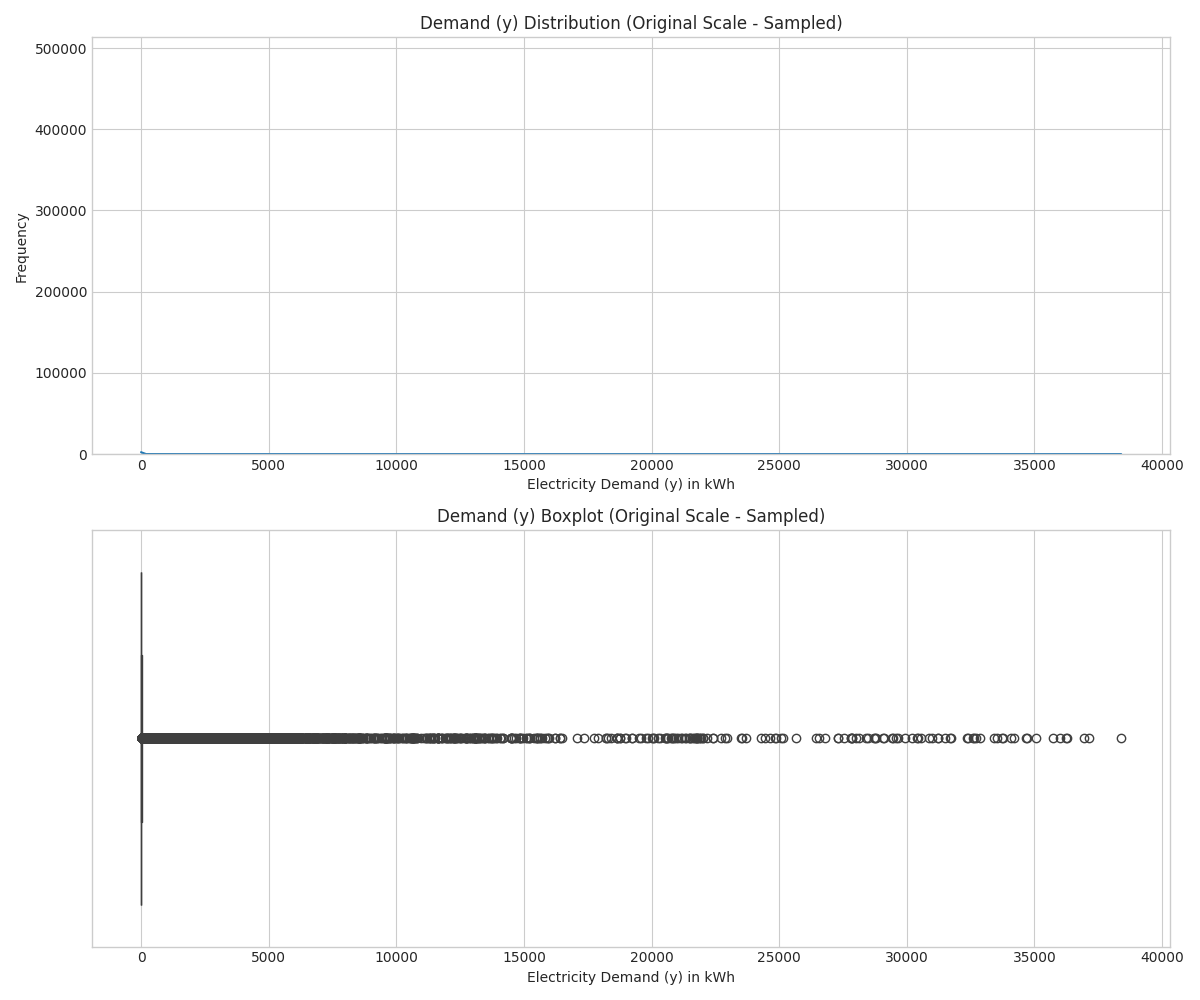
\includegraphics[width=0.8\textwidth]{../plots/demand_y_distribution_original_scale.png}
    \caption{电力需求值 (y) 分布(原始尺度):直方图与箱线图展示了数据的高度右偏特征及大量离群点。} % Updated caption
    \label{fig:demand_y_dist_orig}
\end{figure}

\begin{figure}[H]
    \centering
    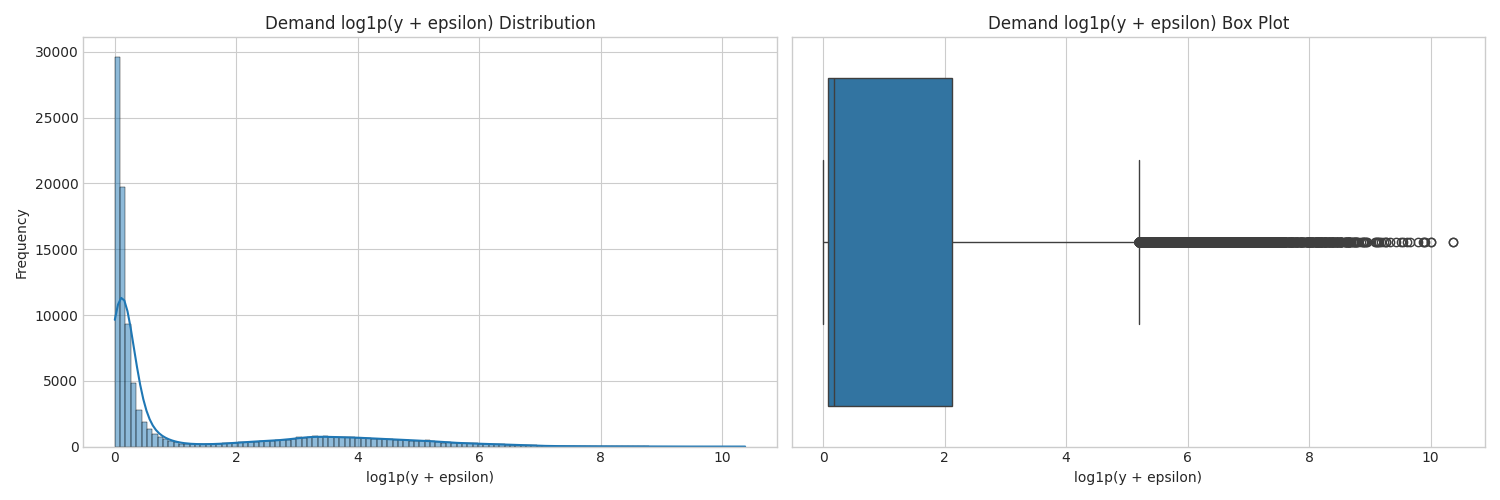
\includegraphics[width=0.8\textwidth]{../plots/demand_y_distribution_log1p_scale.png}
    \caption{电力需求值 (y) 分布(log1p 变换后):对数变换改善了分布的对称性,减少了离群点的影响,但仍可见一定的峰态。} % Updated caption
    \label{fig:demand_y_dist_log}
\end{figure}

\begin{figure}[H]
    \centering
    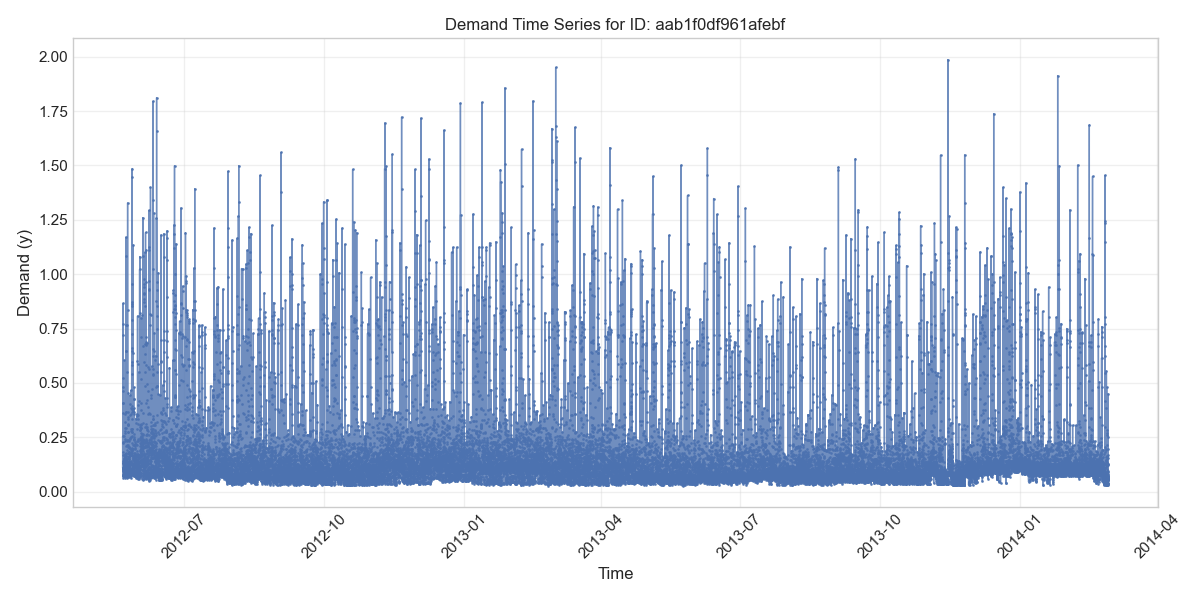
\includegraphics[width=0.8\textwidth]{../plots/timeseries_sample_aab1f0df961afebf.png}
    \caption{电力需求时间序列样本示例 1:展示了典型的日内和周内用电模式。} % Updated caption
    \label{fig:timeseries_sample_1}
\end{figure}

\begin{figure}[H]
    \centering
    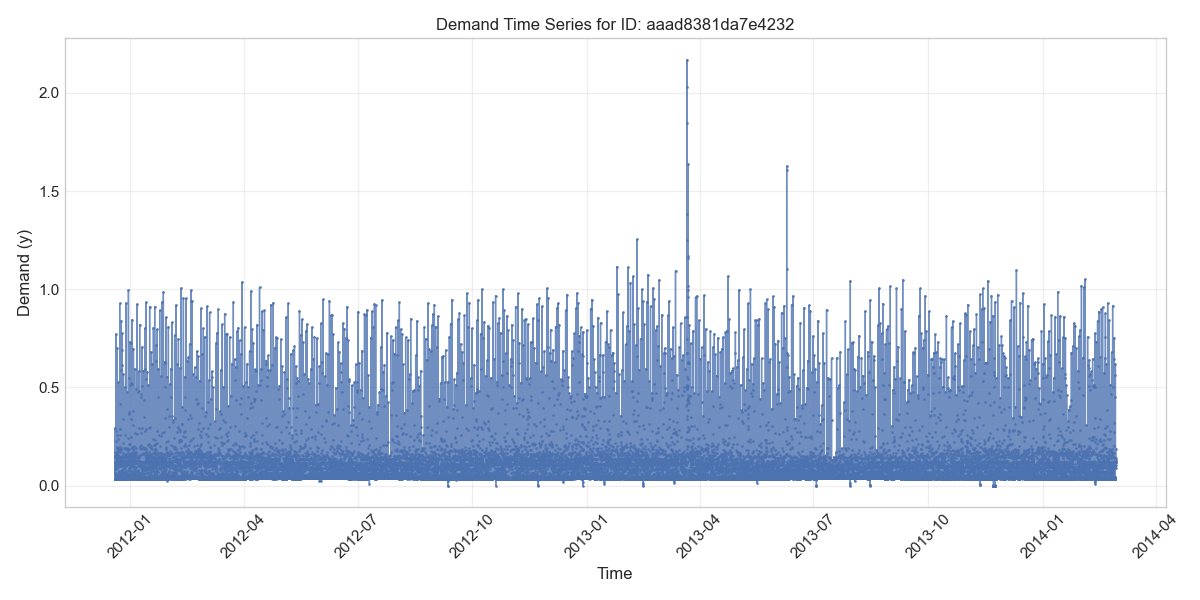
\includegraphics[width=0.8\textwidth]{../plots/timeseries_sample_aaad8381da7e4232.png}
    \caption{电力需求时间序列样本示例 2:可能展示了季节性变化或特定事件的影响。} % Updated caption - more generic as pattern isn't perfectly clear without deeper analysis
    \label{fig:timeseries_sample_2}
\end{figure}

\begin{figure}[H]
    \centering
    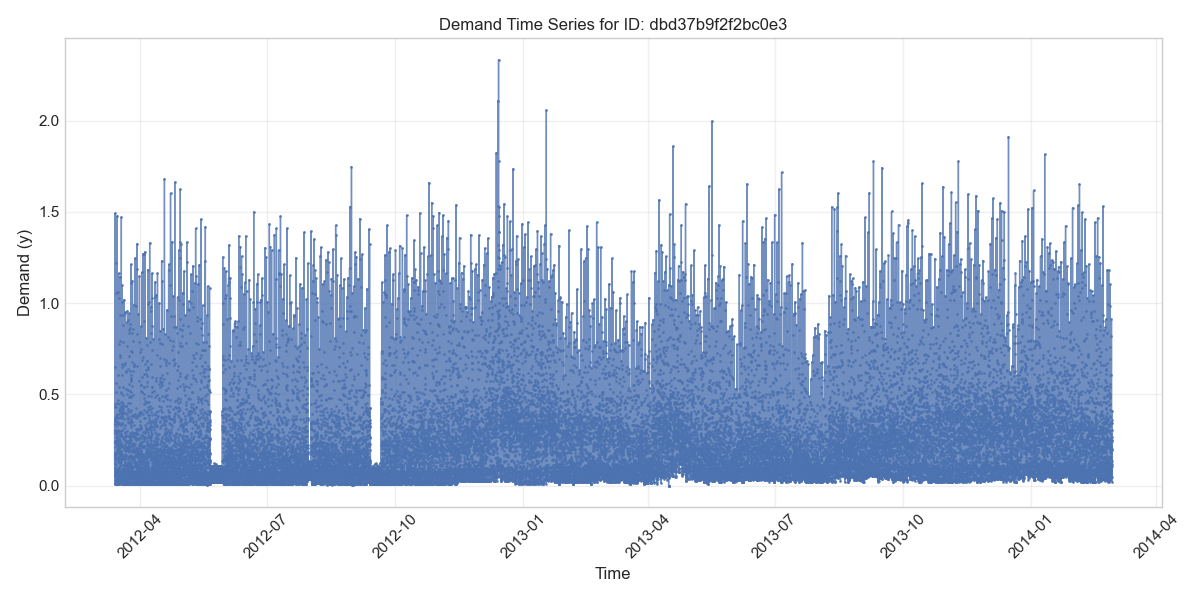
\includegraphics[width=0.8\textwidth]{../plots/timeseries_sample_dbd37b9f2f2bc0e3.png}
    \caption{电力需求时间序列样本示例 3:展示了较为不规则的波动和潜在的异常尖峰值。} % Updated caption
    \label{fig:timeseries_sample_3}
\end{figure}

\begin{figure}[H]
    \centering
    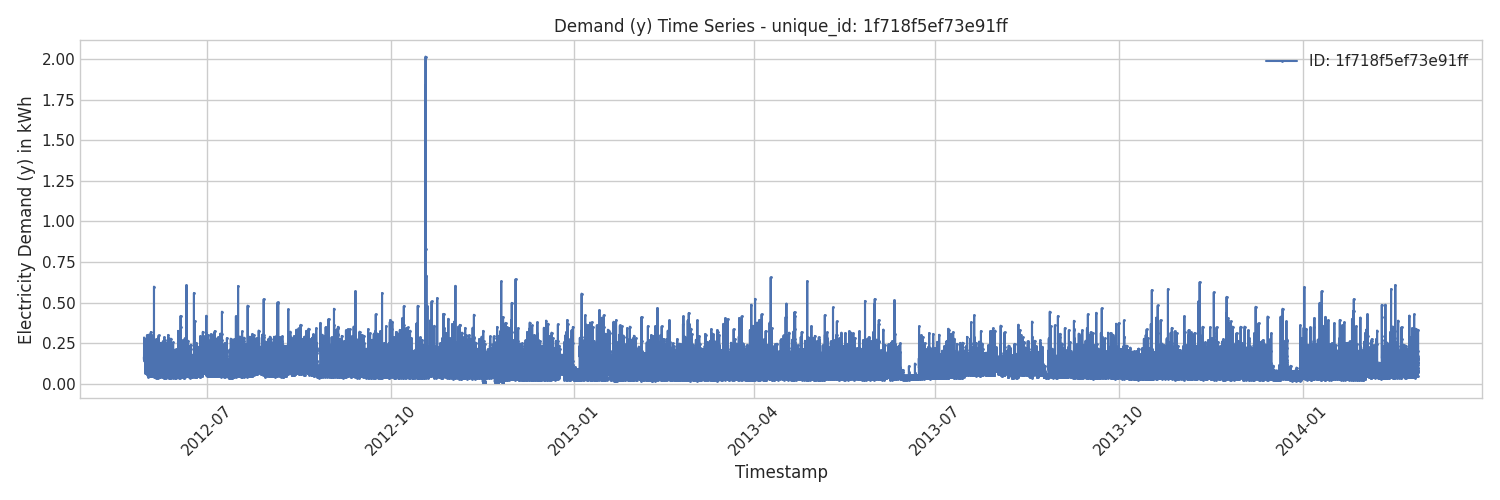
\includegraphics[width=0.8\textwidth]{../plots/timeseries_sample_1f718f5ef73e91ff.png}
    \caption{电力需求时间序列样本示例 4:展示了一个低需求水平用户的用电模式,波动相对较小但仍有周期性。} % Updated caption
    \label{fig:timeseries_sample_4}
\end{figure}

\begin{figure}[H]
    \centering
    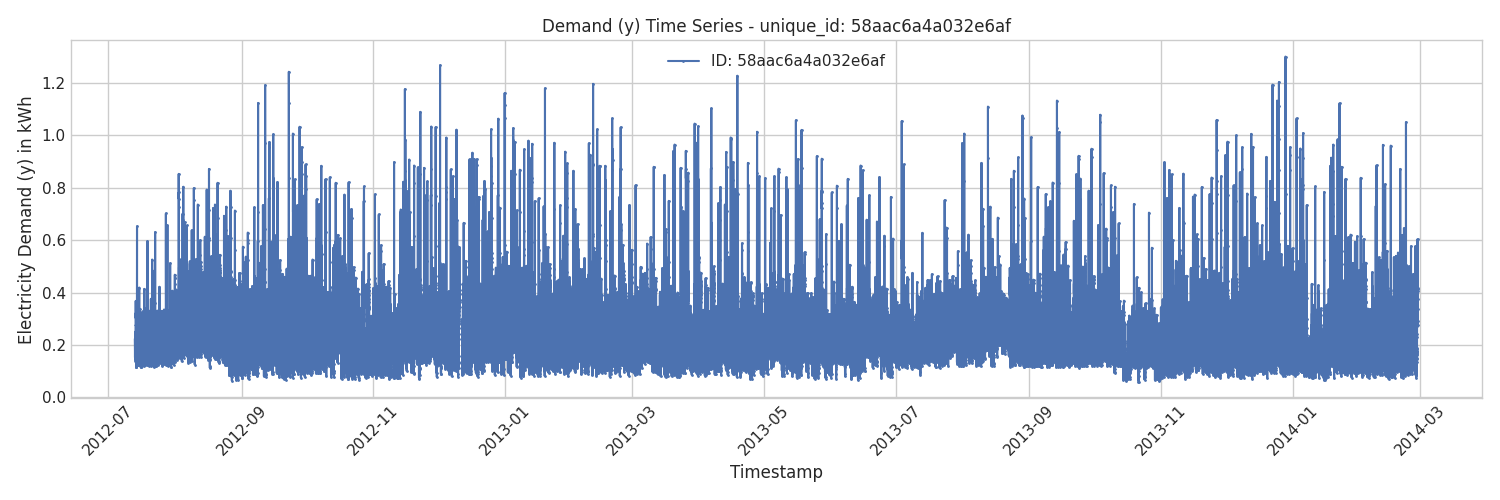
\includegraphics[width=0.8\textwidth]{../plots/timeseries_sample_58aac6a4a032e6af.png}
    \caption{电力需求时间序列样本示例 5:清晰地展示了工作日与周末之间显著不同的用电模式。} % Updated caption
    \label{fig:timeseries_sample_5}
\end{figure}

\begin{figure}[H]
    \centering
    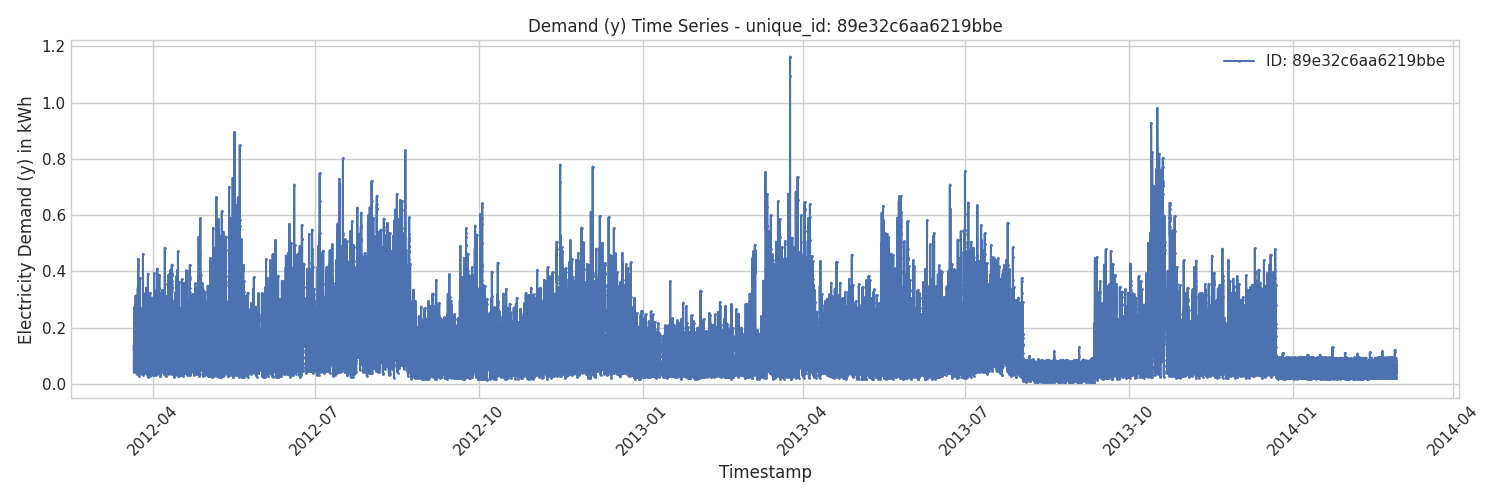
\includegraphics[width=0.8\textwidth]{../plots/timeseries_sample_89e32c6aa6219bbe.png}
    \caption{电力需求时间序列样本示例 6:序列中包含了一些显著的、可能是由特殊事件引起的用电峰值。} % Updated caption
    \label{fig:timeseries_sample_6}
\end{figure}

\begin{figure}[H]
    \centering
    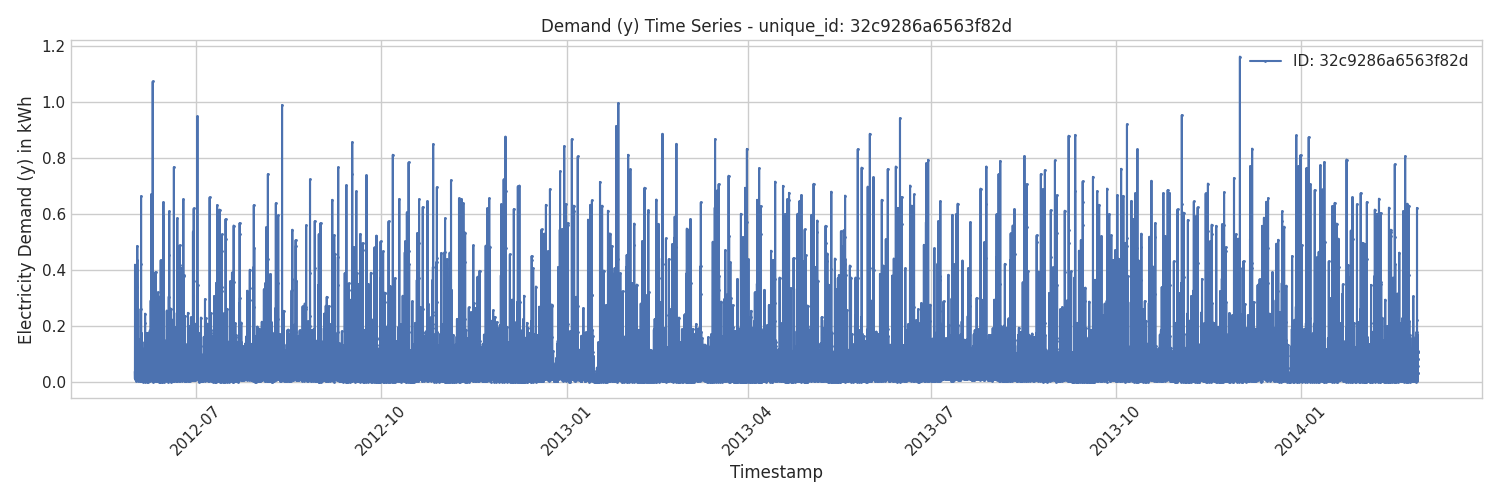
\includegraphics[width=0.8\textwidth]{../plots/timeseries_sample_32c9286a6563f82d.png}
    \caption{电力需求时间序列样本示例 7:可能展示了包含长期趋势变化或模式转变的用电情况。} % Updated caption
    \label{fig:timeseries_sample_7}
\end{figure}

\section{元数据分析}
\label{sec:metadata_analysis}

本节分析了提供监测点静态属性的元数据。

对关键的分类特征(如建筑类型、地理位置名称、数据采样频率、时区、原始数据集来源)进行了频率统计,并通过条形图(如图 \ref{fig:metadata_dist_building_class} 至 \ref{fig:metadata_dist_dataset})展示其分布。主要发现包括:建筑类型以住宅为主;地理位置高度集中于伦敦地区;存在多种数据采样频率,以 30 分钟和 1 小时为主;大部分数据时区为欧洲/伦敦,且主要来源于少数几个数据集。

对于数值型元数据(如经纬度坐标、集群规模),计算了其描述性统计量,并绘制了直方图(如图 \ref{fig:metadata_hist_latitude}, \ref{fig:metadata_hist_longitude}, \ref{fig:metadata_hist_cluster_size})和散点图(如图 \ref{fig:metadata_location_scatter})来观察其分布和空间聚集特性。分析确认了地理位置的集中性,并了解了监测点所代表的建筑集群规模的分布情况。同时,对地理位置信息缺失的记录进行了特征探查。

\begin{figure}[H]
    \centering
    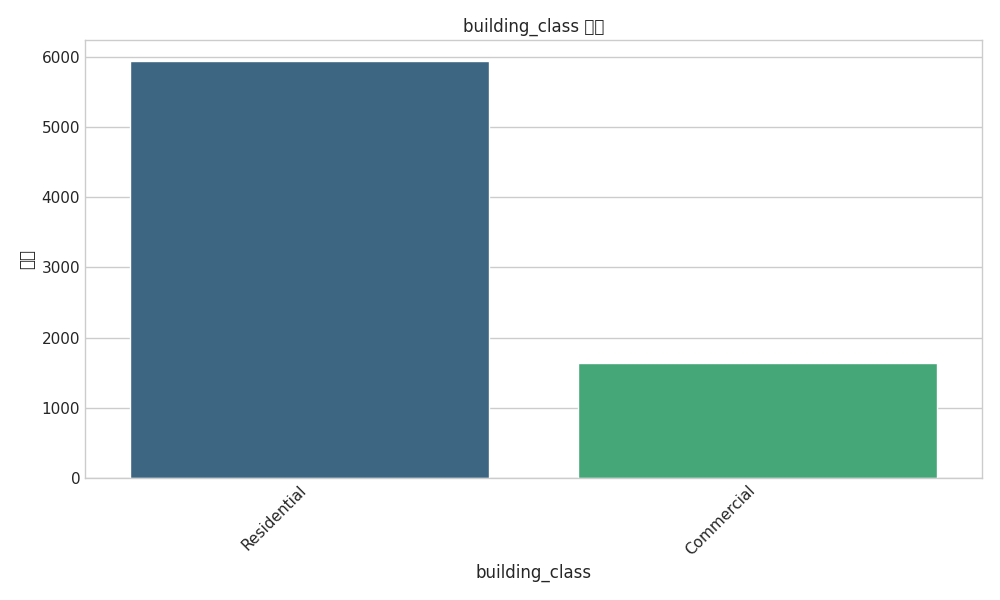
\includegraphics[width=0.6\textwidth]{../plots/metadata_dist_building_class.png}
    \caption{元数据:建筑类型 (building\_class) 分布,显示住宅类远多于商业类。} % Updated caption
    \label{fig:metadata_dist_building_class}
\end{figure}

\begin{figure}[H]
    \centering
    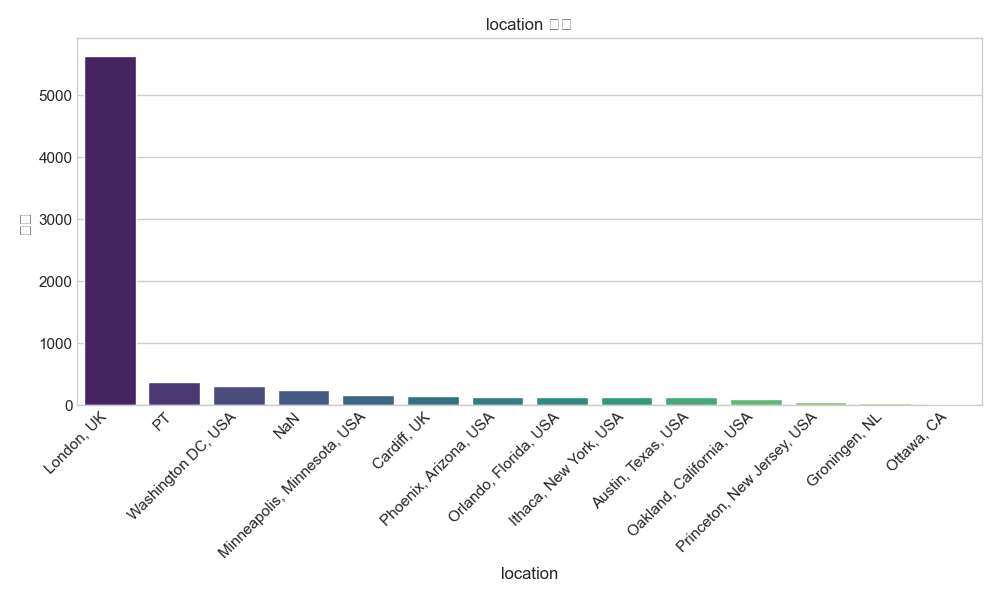
\includegraphics[width=0.8\textwidth]{../plots/metadata_dist_location.png}
    \caption{元数据:地理位置 (location) 分布(频率最高的 Top N 地点),显示数据主要集中于伦敦。} % Updated caption
    \label{fig:metadata_dist_location}
\end{figure}

\begin{figure}[H]
    \centering
    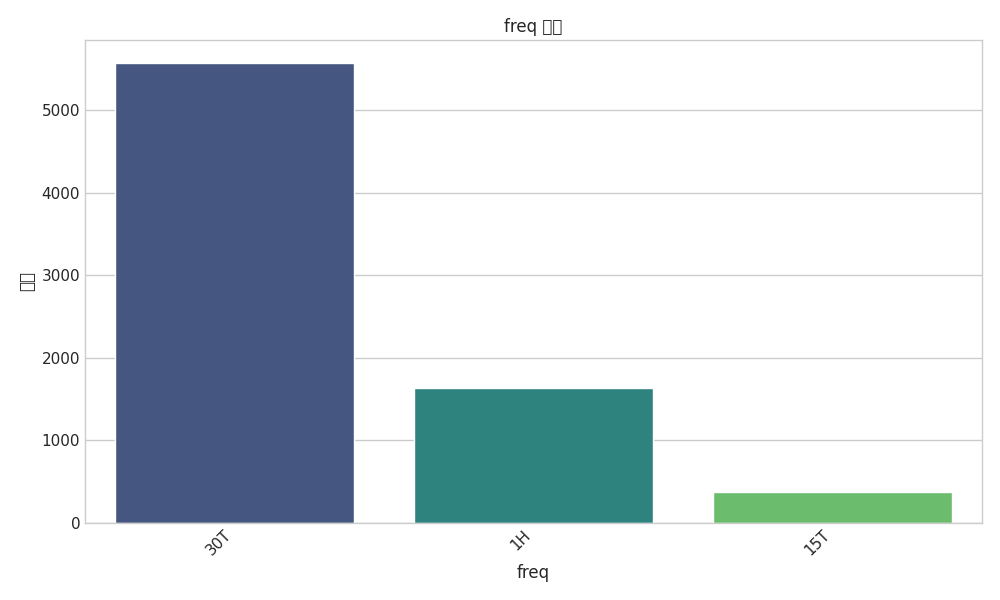
\includegraphics[width=0.6\textwidth]{../plots/metadata_dist_freq.png}
    \caption{元数据:数据采样频率 (freq) 分布,以 30 分钟和 1 小时为主。} % Updated caption
    \label{fig:metadata_dist_freq}
\end{figure}

\begin{figure}[H]
    \centering
    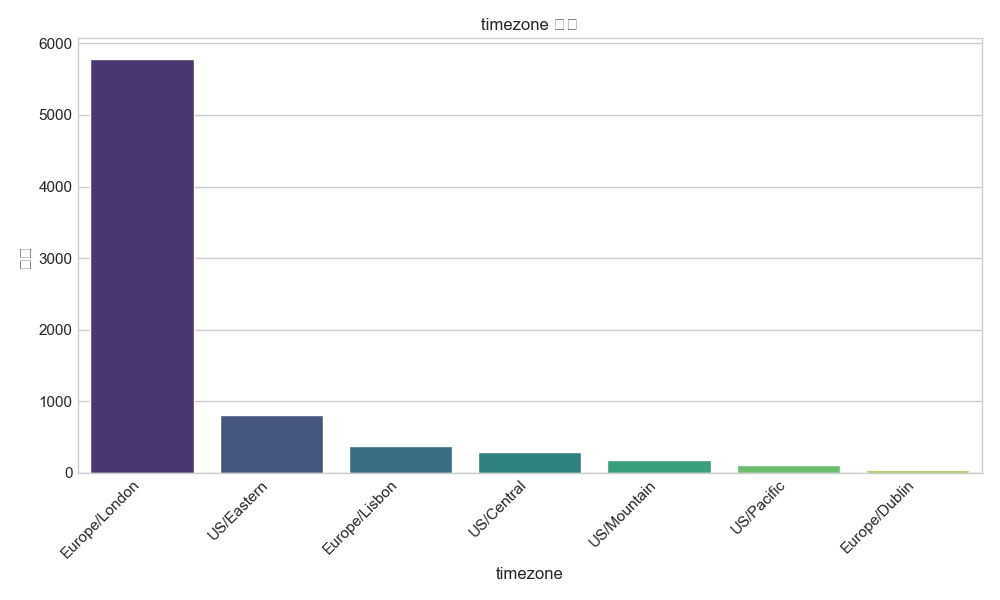
\includegraphics[width=0.7\textwidth]{../plots/metadata_dist_timezone.png}
    \caption{元数据:时区 (timezone) 分布,主要为欧洲/伦敦时区。} % Updated caption
    \label{fig:metadata_dist_timezone}
\end{figure}

\begin{figure}[H]
    \centering
    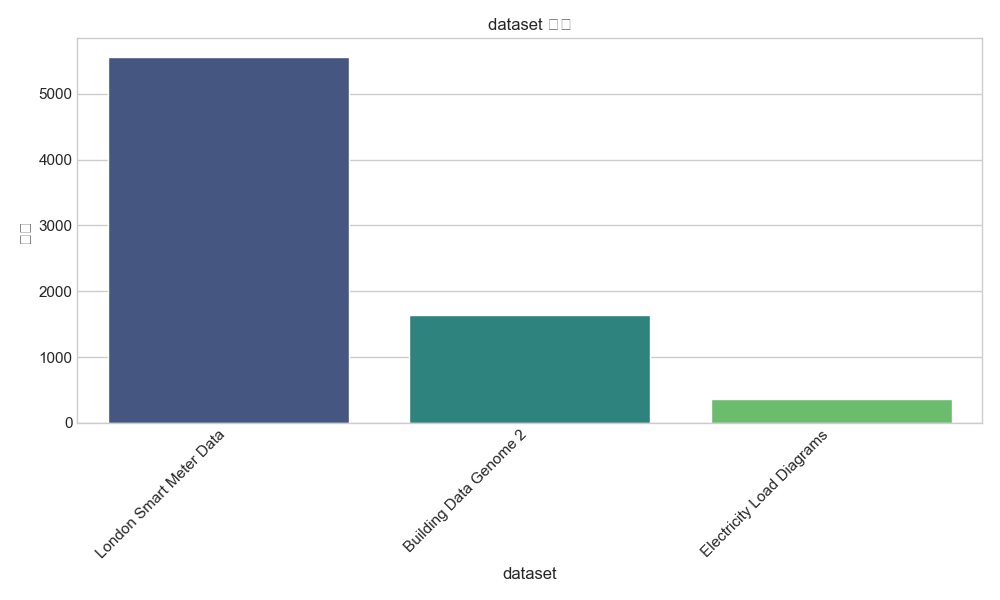
\includegraphics[width=0.7\textwidth]{../plots/metadata_dist_dataset.png}
    \caption{元数据:原始数据集来源 (dataset) 分布,显示主要来源。} % Updated caption
    \label{fig:metadata_dist_dataset}
\end{figure}

\begin{figure}[H]
    \centering
    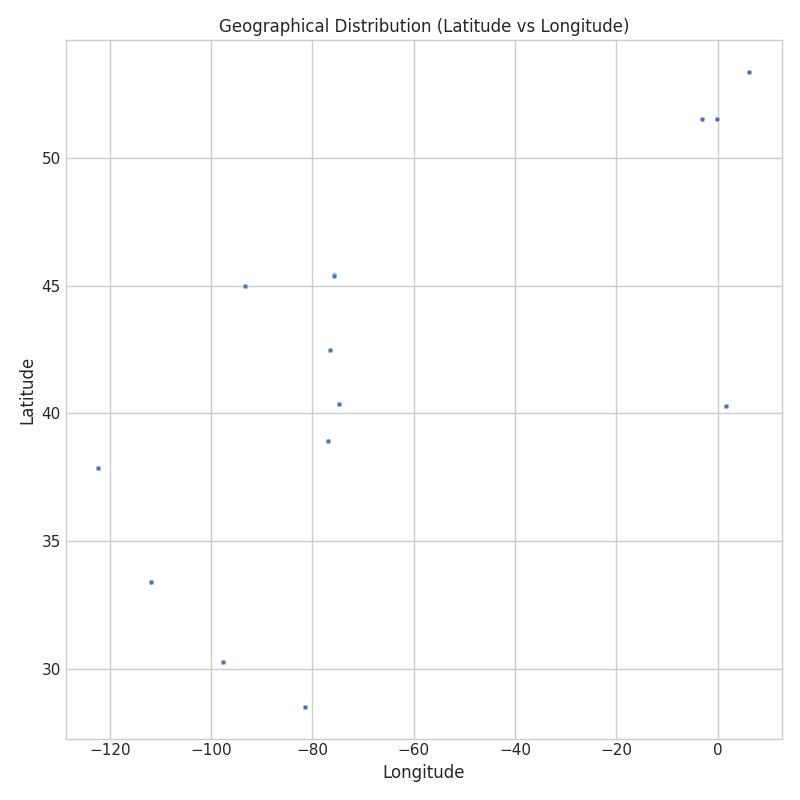
\includegraphics[width=0.7\textwidth]{../plots/metadata_location_scatter.png}
    \caption{元数据:监测点地理位置散点图(经度 vs 纬度),直观展示空间分布。} % Updated caption
    \label{fig:metadata_location_scatter}
\end{figure}

\begin{figure}[H]
    \centering
    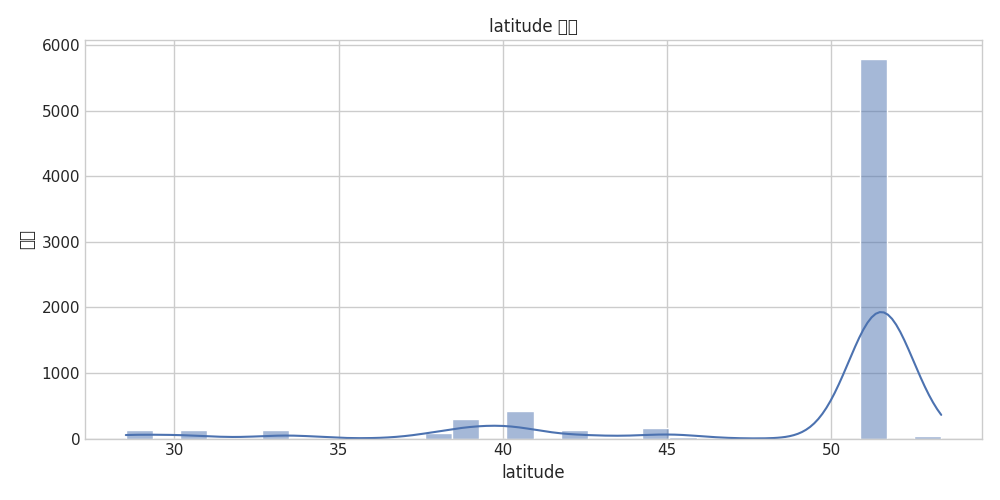
\includegraphics[width=0.7\textwidth]{../plots/metadata_hist_latitude.png}
    \caption{元数据:纬度 (latitude) 分布直方图,反映监测点在纬度上的分布情况。} % Updated caption
    \label{fig:metadata_hist_latitude}
\end{figure}

\begin{figure}[H]
    \centering
    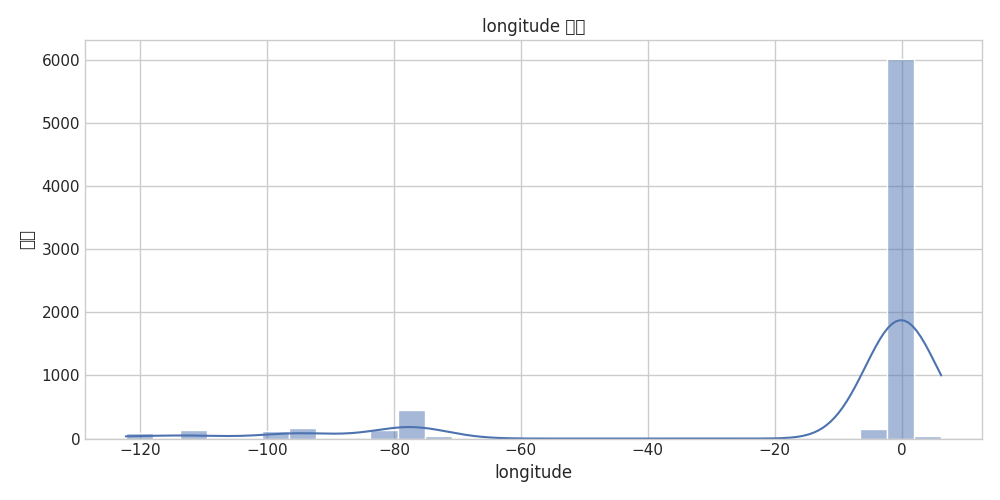
\includegraphics[width=0.7\textwidth]{../plots/metadata_hist_longitude.png}
    \caption{元数据:经度 (longitude) 分布直方图,反映监测点在经度上的分布情况。} % Updated caption
    \label{fig:metadata_hist_longitude}
\end{figure}

\begin{figure}[H]
    \centering
    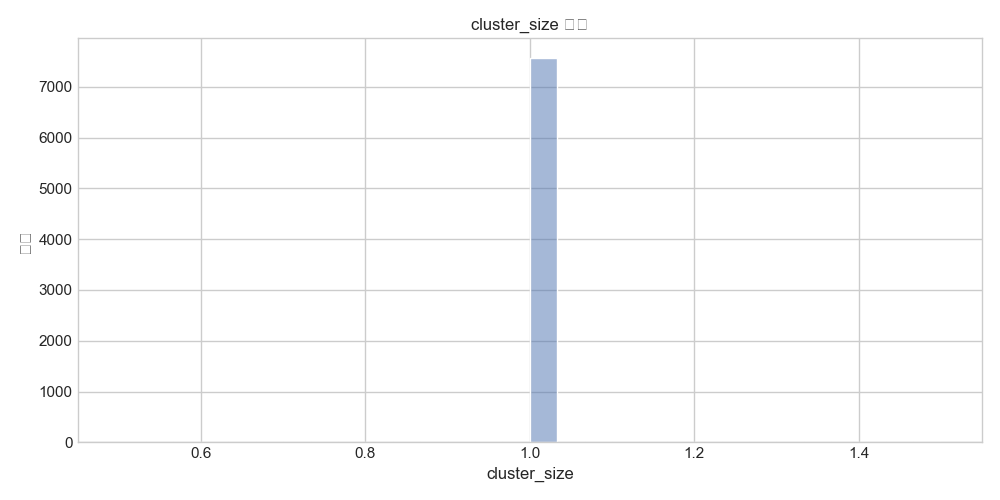
\includegraphics[width=0.7\textwidth]{../plots/metadata_hist_cluster_size.png}
    \caption{元数据:集群规模 (cluster\_size) 分布直方图,显示多数监测点代表单个建筑。} % Updated caption
    \label{fig:metadata_hist_cluster_size}
\end{figure}

\section{天气数据分析}
\label{sec:weather_analysis}

本节对可能影响电力需求的环境因素——天气数据进行了分析。

\subsection{基本天气特征分析}
\label{subsec:basic_weather}
计算了关键数值型天气变量(如温度、相对湿度、降水量、风速等)的描述性统计量,了解其基本范围和集中趋势。

\subsection{主要天气变量分布}
\label{subsec:major_weather_dist}
通过绘制直方图或核密度图,可视化了主要天气变量的分布特征(如图 \ref{fig:weather_dist_temp} 至 \ref{fig:weather_dist_apparent_temp} 等)。分析涵盖了温度与湿度、降水与积雪、云量与辐射、大气压力、土壤特性以及风速与风向等多个方面。同时,对部分变量(如降水量相关变量)进行了非负值检查,确认数据记录的合理性。

\subsection{分类天气特征分析}
\label{subsec:categorical_weather}
分析了重要的分类天气特征的分布,包括描述综合天气状况的天气代码(图 \ref{fig:weather_dist_code})和区分白天/夜晚的标识(图 \ref{fig:weather_dist_is_day})。

\begin{figure}[H]
    \centering
    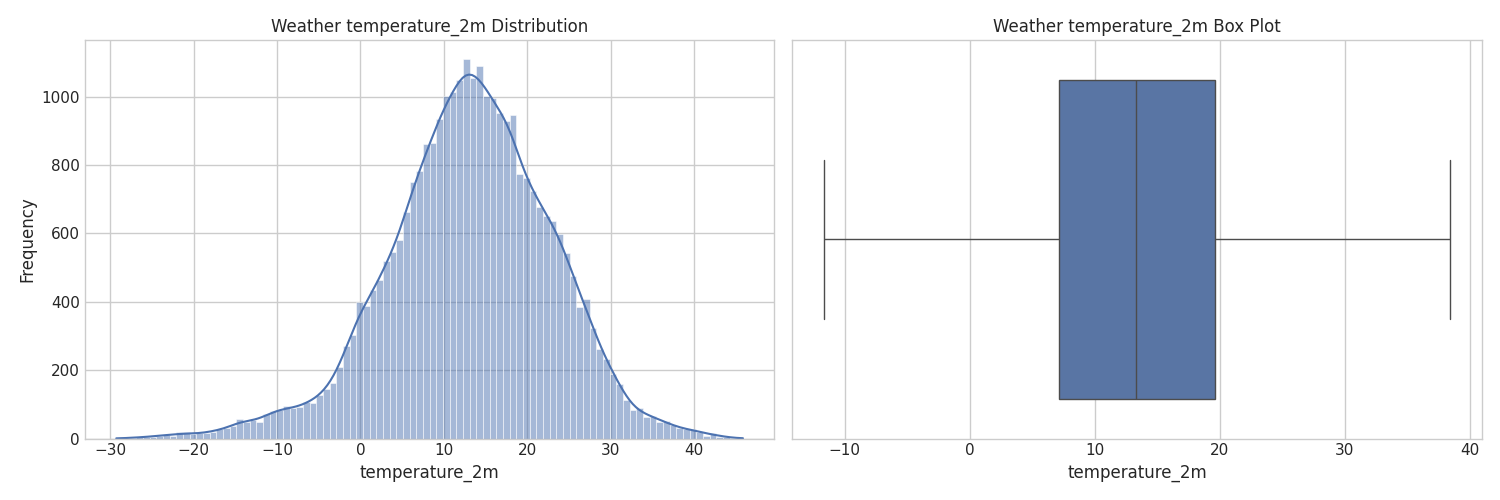
\includegraphics[width=0.8\textwidth]{../plots/weather_distribution_temperature_2m.png}
    \caption{天气分析:2 米高度温度 (temperature\_2m) 分布,呈近似正态分布。} % Updated caption
    \label{fig:weather_dist_temp}
\end{figure}

\begin{figure}[H]
    \centering
    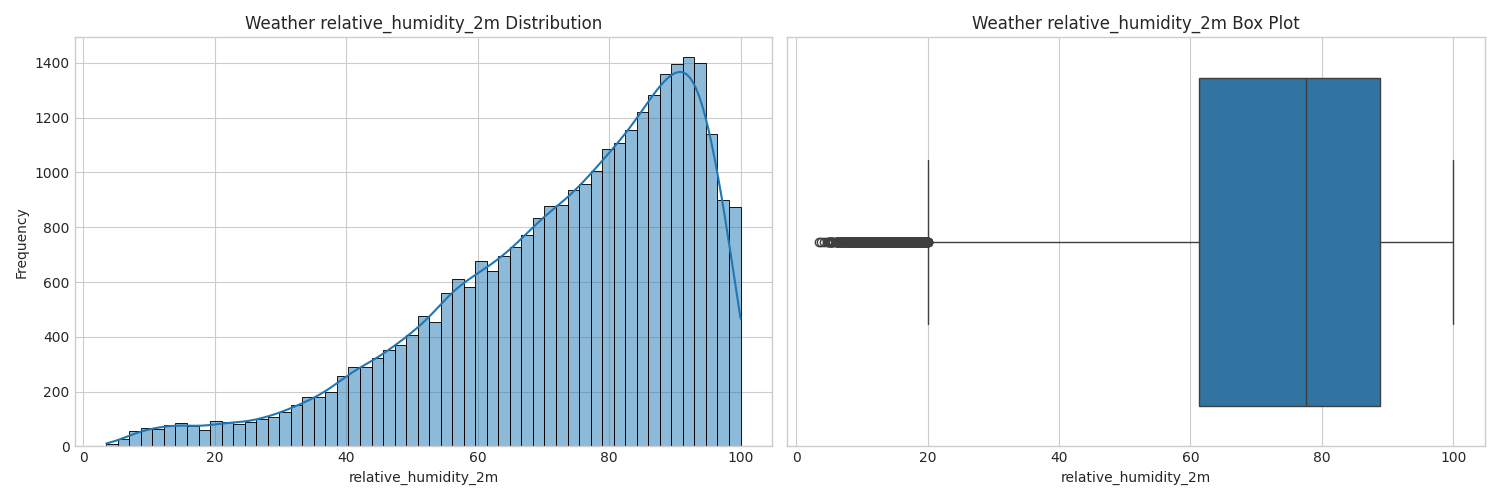
\includegraphics[width=0.8\textwidth]{../plots/weather_distribution_relative_humidity_2m.png}
    \caption{天气分析:2 米高度相对湿度 (relative\_humidity\_2m) 分布,范围较广,倾向于较高湿度。} % Updated caption
    \label{fig:weather_dist_humidity}
\end{figure}

\begin{figure}[H]
    \centering
    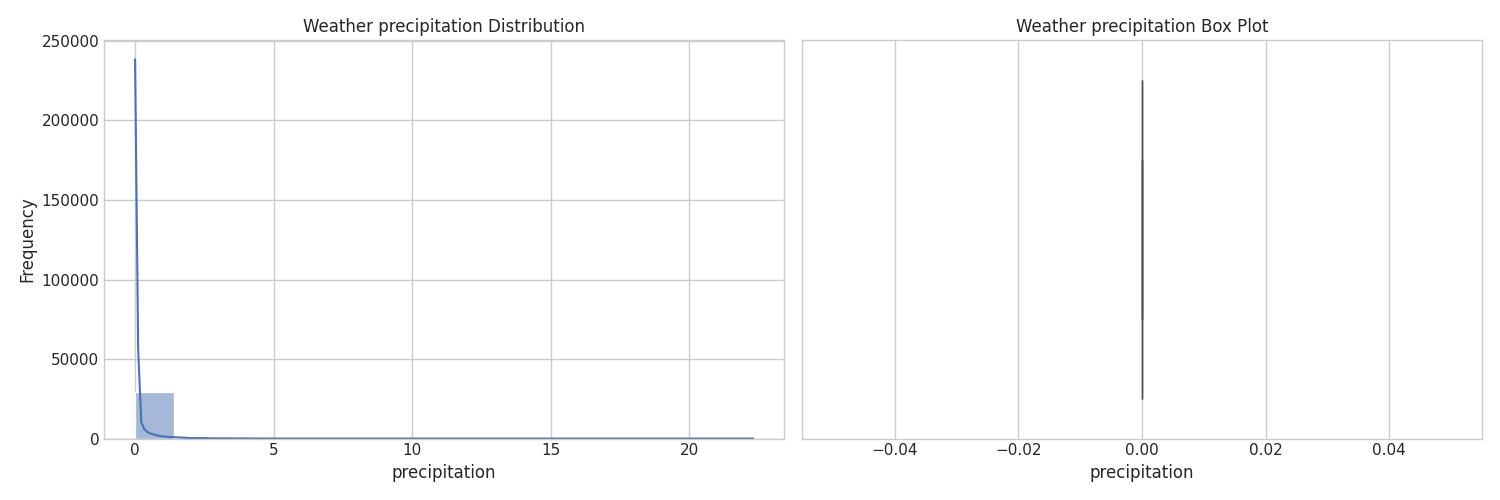
\includegraphics[width=0.8\textwidth]{../plots/weather_distribution_precipitation.png}
    \caption{天气分析:总降水量 (precipitation) 分布,典型的零膨胀和右偏分布。} % Updated caption
    \label{fig:weather_dist_precip}
\end{figure}

\begin{figure}[H]
    \centering
    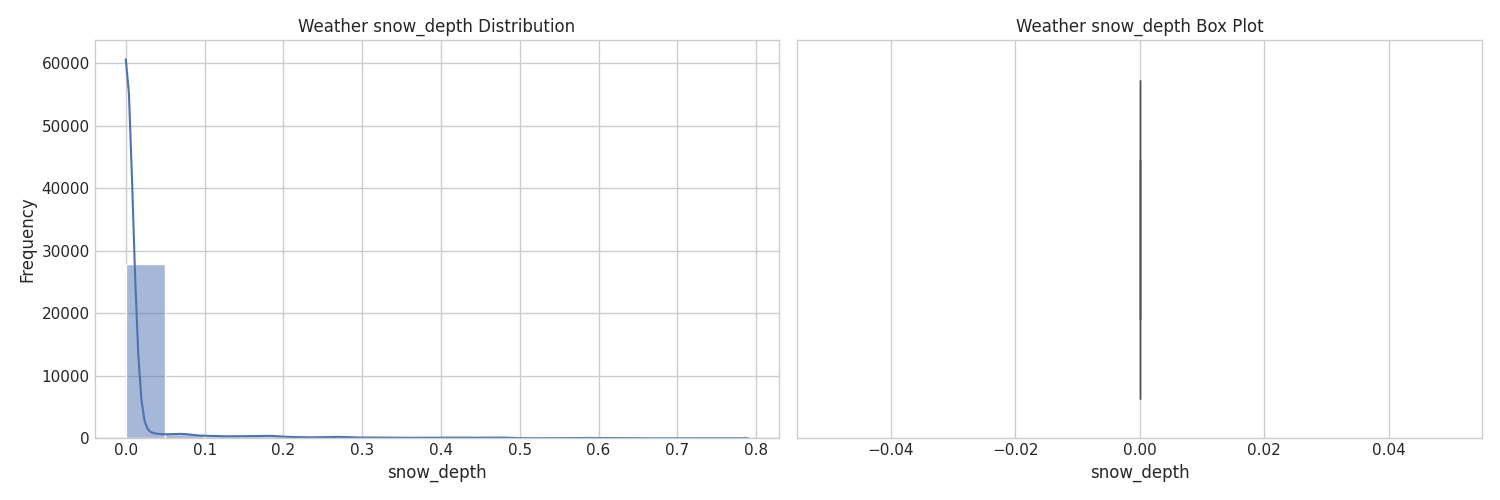
\includegraphics[width=0.8\textwidth]{../plots/weather_distribution_snow_depth.png}
    \caption{天气分析:积雪深度 (snow\_depth) 分布,绝大多数时间为零,少数时间有积雪。} % Updated caption
    \label{fig:weather_dist_snow}
\end{figure}

\begin{figure}[H]
    \centering
    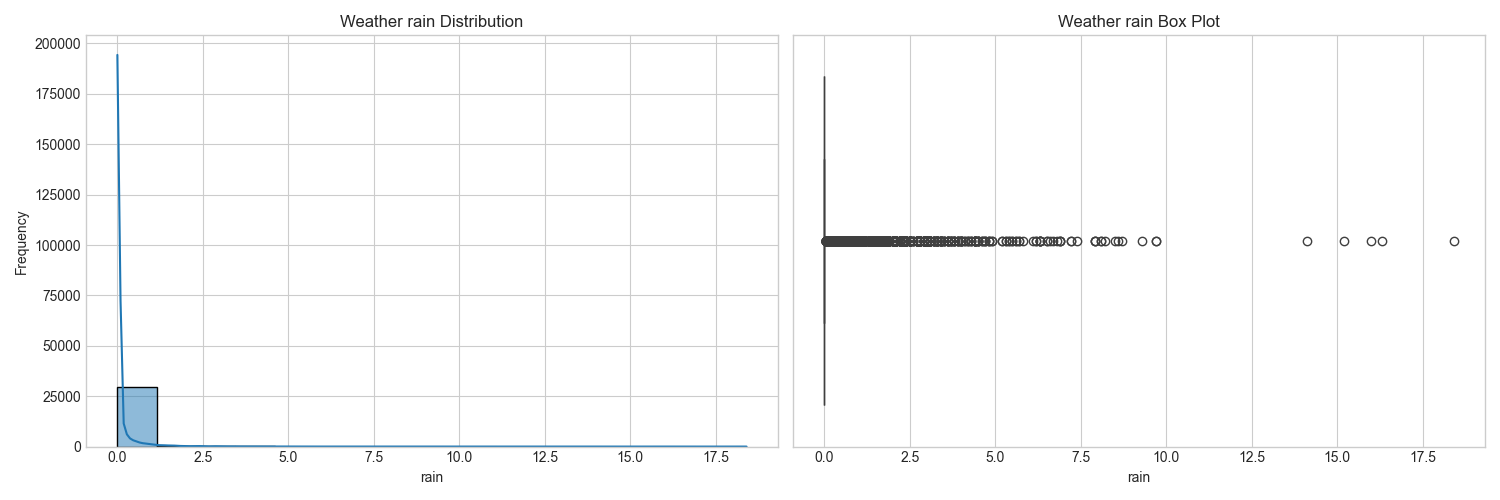
\includegraphics[width=0.8\textwidth]{../plots/weather_distribution_rain.png}
    \caption{天气分析:降雨量 (rain) 分布,与总降水量类似,零膨胀且右偏。} % Updated caption
    \label{fig:weather_dist_rain}
\end{figure}

\begin{figure}[H]
    \centering
    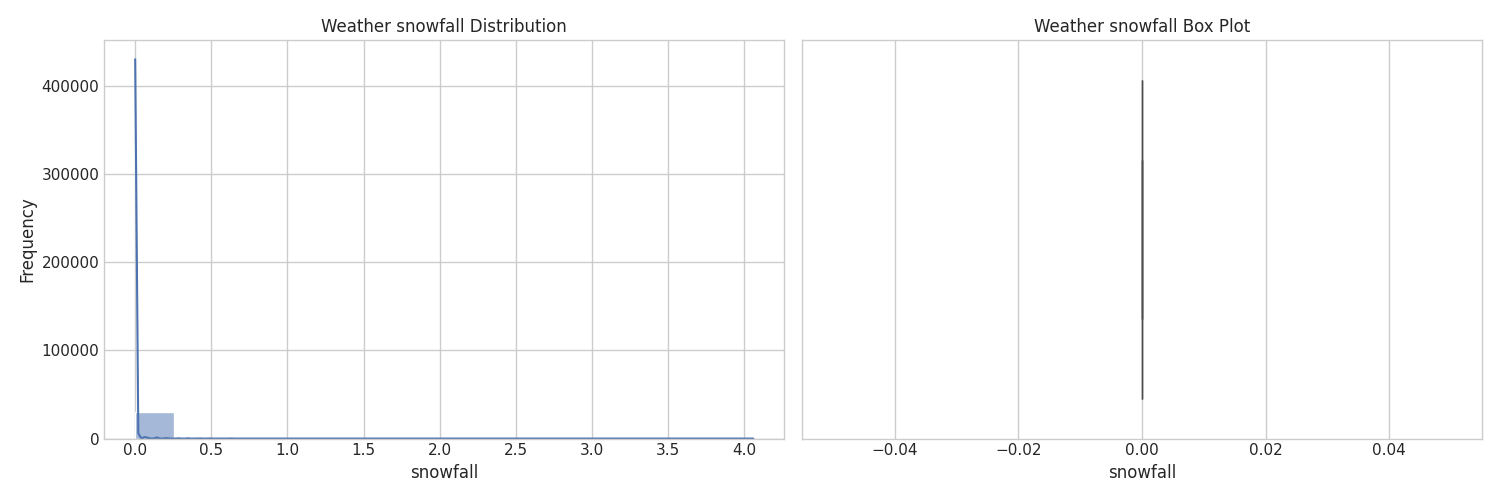
\includegraphics[width=0.8\textwidth]{../plots/weather_distribution_snowfall.png}
    \caption{天气分析:降雪量 (snowfall) 分布,零膨胀且右偏,发生频率低于降雨。} % Updated caption
    \label{fig:weather_dist_snowfall}
\end{figure}

\begin{figure}[H]
    \centering
    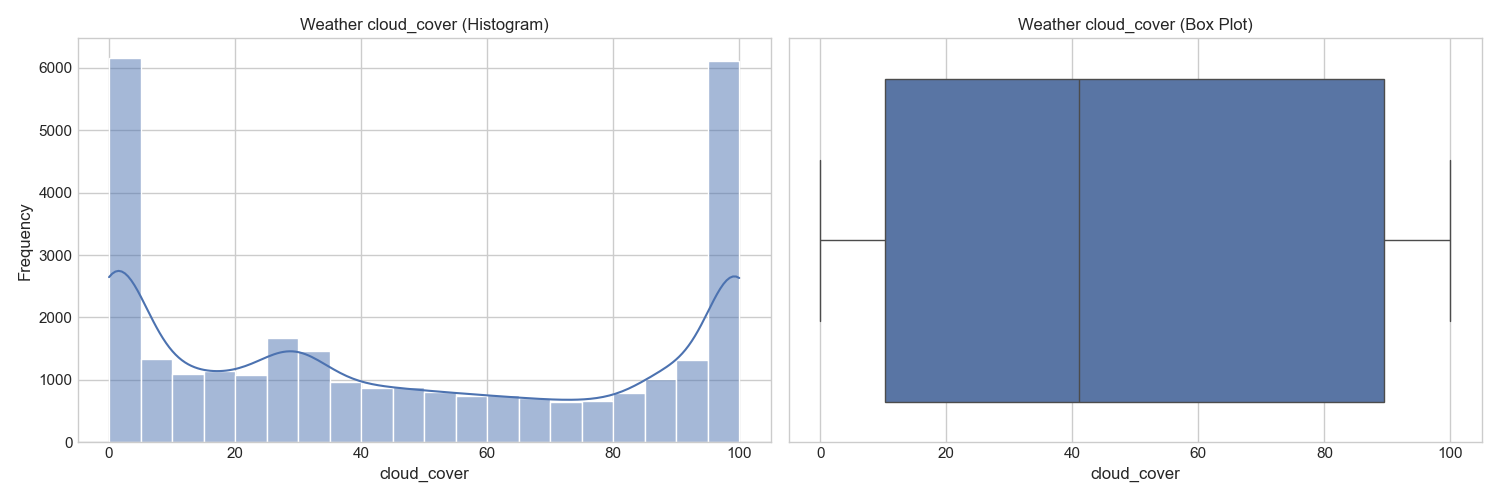
\includegraphics[width=0.8\textwidth]{../plots/weather_distribution_cloud_cover.png}
    \caption{天气分析:总云量 (cloud\_cover) 分布,呈现两端高中间低的 U 形分布特征。} % Updated caption
    \label{fig:weather_dist_cloud}
\end{figure}

\begin{figure}[H]
    \centering
    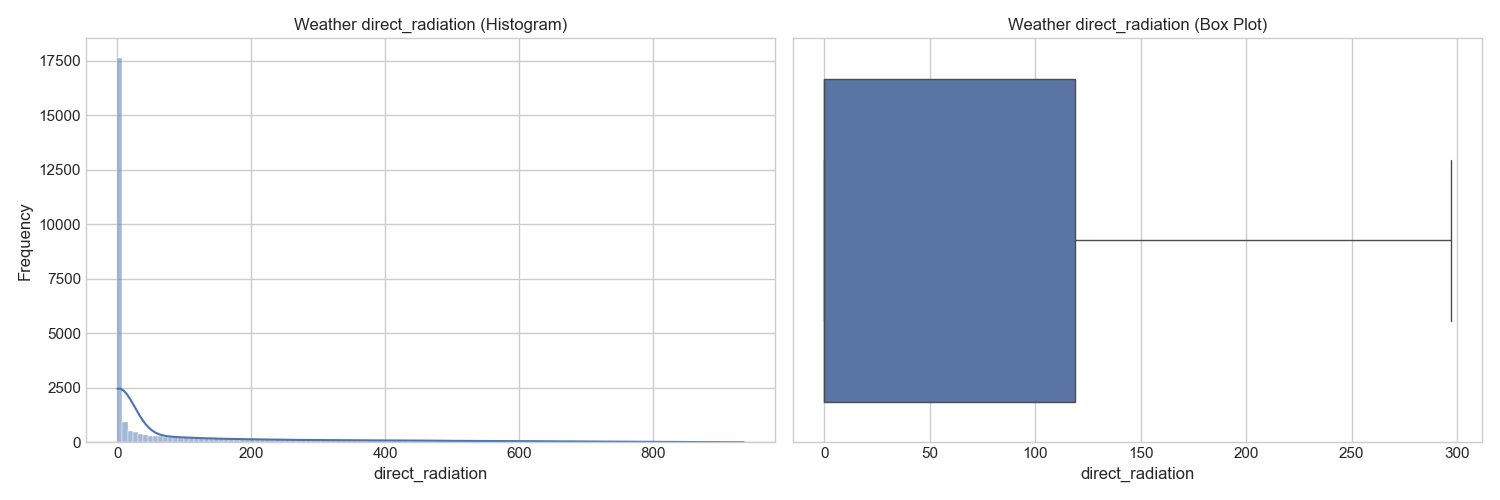
\includegraphics[width=0.8\textwidth]{../plots/weather_distribution_direct_radiation.png}
    \caption{天气分析:直接辐射 (direct\_radiation) 分布,零膨胀且右偏,反映日照强度。} % Updated caption
    \label{fig:weather_dist_radiation}
\end{figure}

\begin{figure}[H]
    \centering
    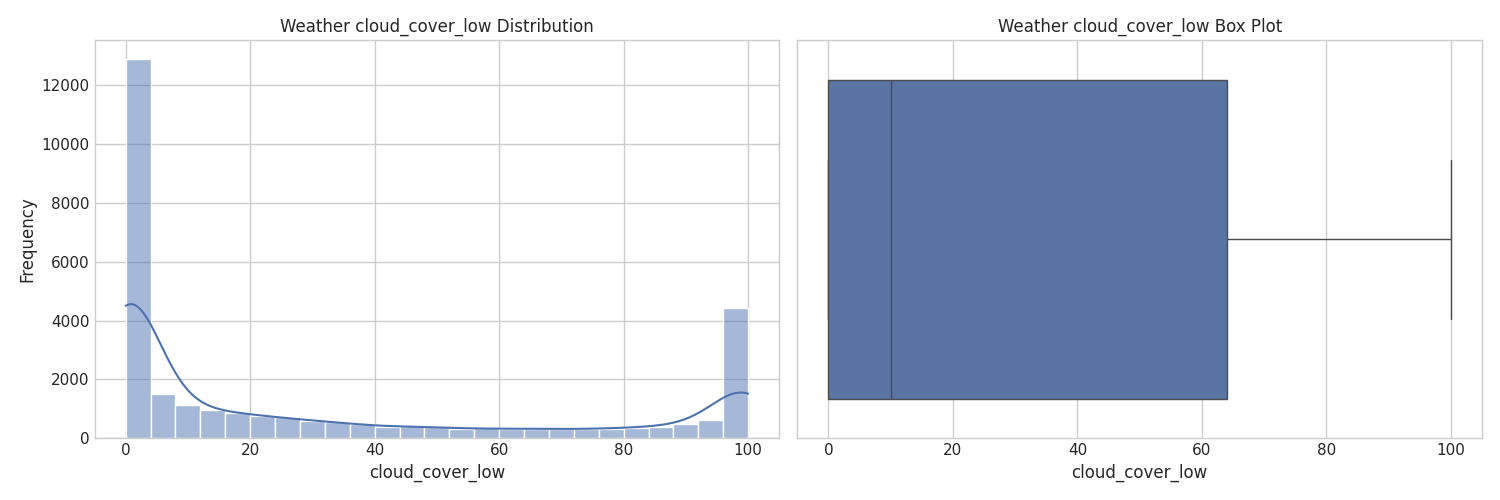
\includegraphics[width=0.8\textwidth]{../plots/weather_distribution_cloud_cover_low.png}
    \caption{天气分析:低空云量 (cloud\_cover\_low) 分布,同样常见于全覆盖或无覆盖状态。} % Updated caption
    \label{fig:weather_dist_cloud_low}
\end{figure}

\begin{figure}[H]
    \centering
    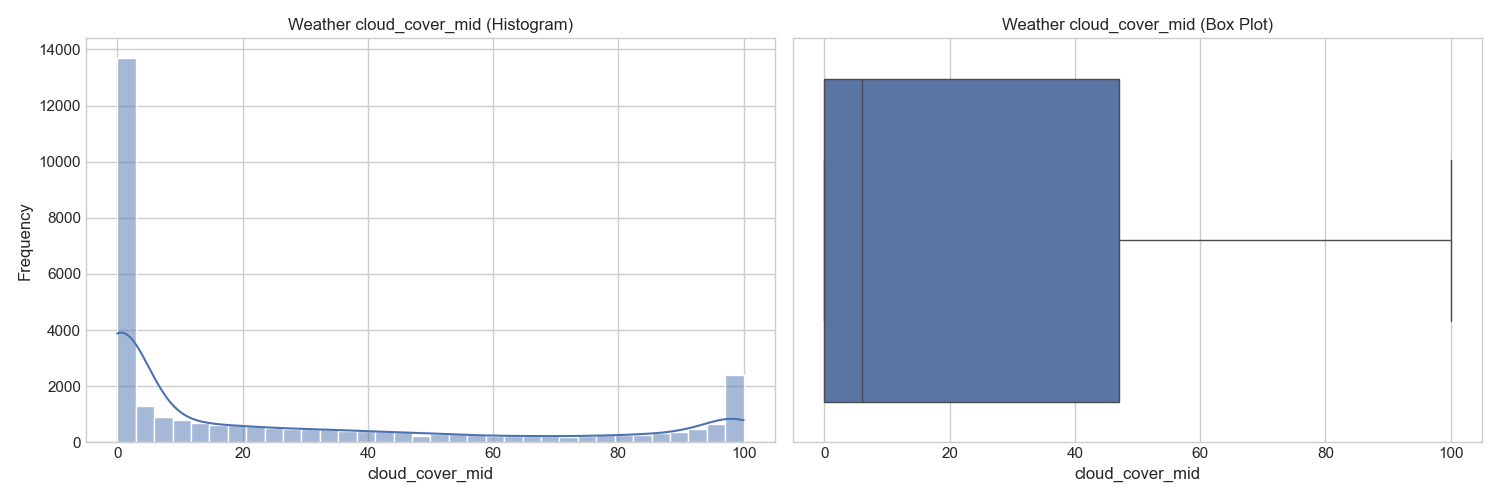
\includegraphics[width=0.8\textwidth]{../plots/weather_distribution_cloud_cover_mid.png}
    \caption{天气分析:中空云量 (cloud\_cover\_mid) 分布,相对低云和高云,中间覆盖度比例稍高。} % Updated caption
    \label{fig:weather_dist_cloud_mid}
\end{figure}

\begin{figure}[H]
    \centering
    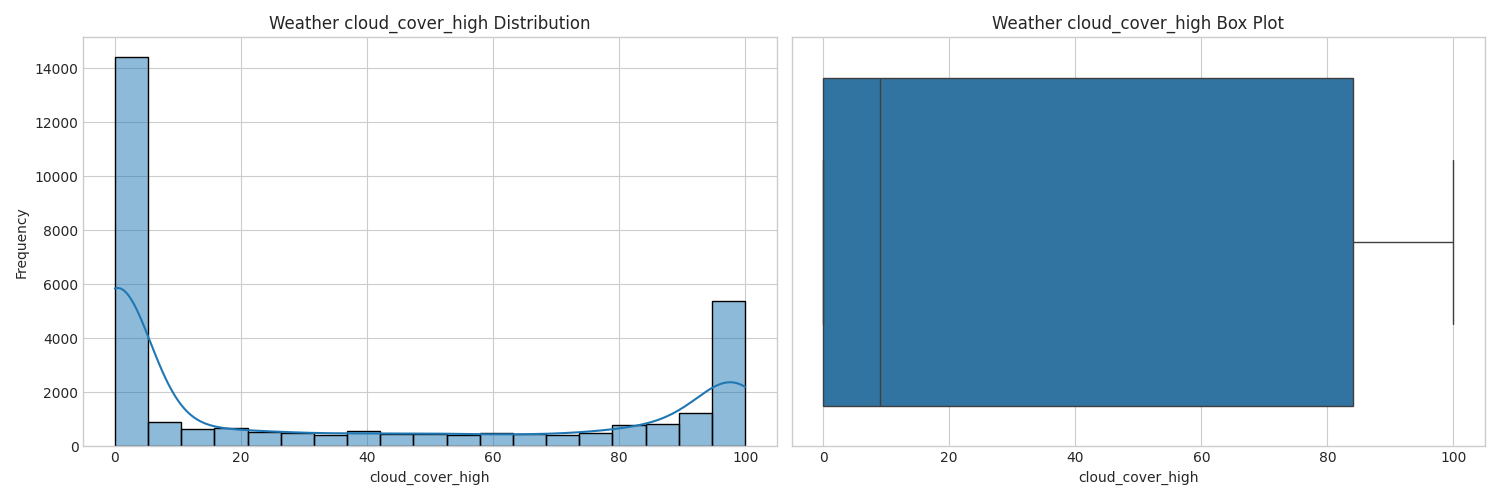
\includegraphics[width=0.8\textwidth]{../plots/weather_distribution_cloud_cover_high.png}
    \caption{天气分析:高空云量 (cloud\_cover\_high) 分布,与低云类似,常见于两极状态。} % Updated caption
    \label{fig:weather_dist_cloud_high}
\end{figure}

\begin{figure}[H]
    \centering
    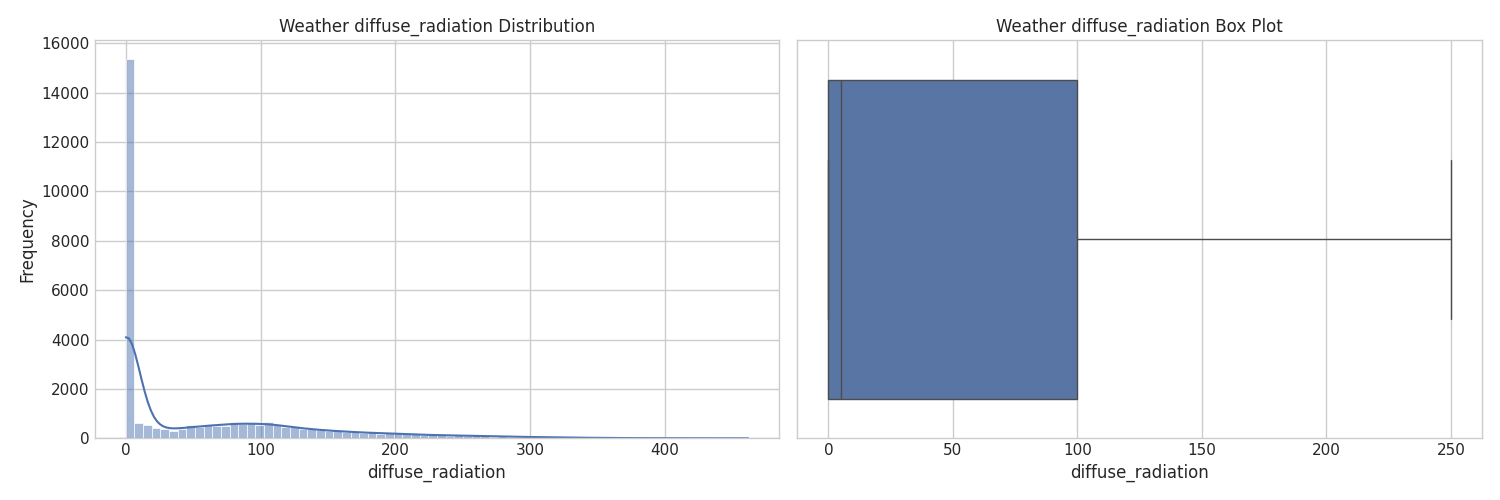
\includegraphics[width=0.8\textwidth]{../plots/weather_distribution_diffuse_radiation.png}
    \caption{天气分析:漫射辐射 (diffuse\_radiation) 分布,零膨胀且右偏。} % Updated caption
    \label{fig:weather_dist_diffuse_radiation}
\end{figure}

\begin{figure}[H]
    \centering
    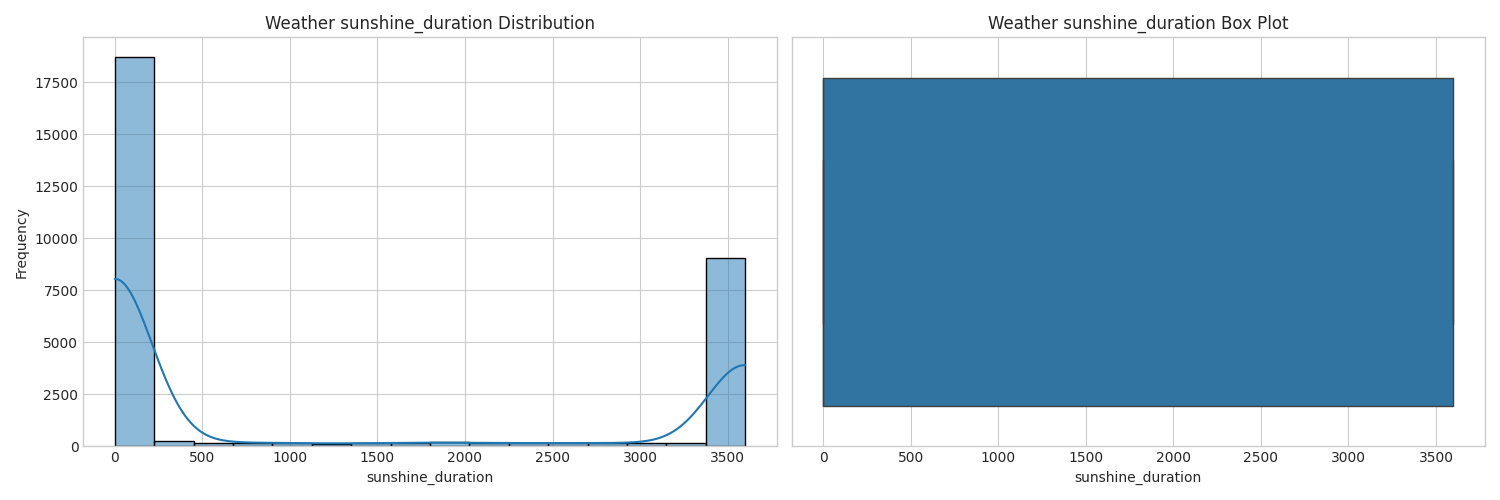
\includegraphics[width=0.8\textwidth]{../plots/weather_distribution_sunshine_duration.png}
    \caption{天气分析:日照时长 (sunshine\_duration) 分布,呈现两极分化,要么无日照,要么接近满时长。} % Updated caption
    \label{fig:weather_dist_sunshine}
\end{figure}

\begin{figure}[H]
    \centering
    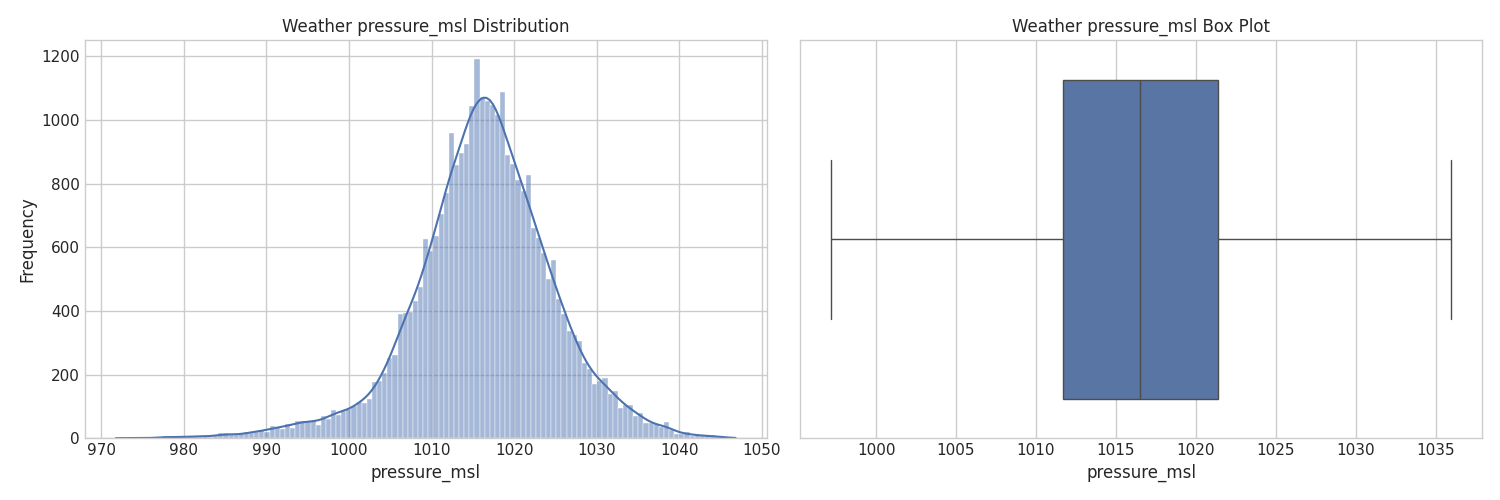
\includegraphics[width=0.8\textwidth]{../plots/weather_distribution_pressure_msl.png}
    \caption{天气分析:海平面气压 (pressure\_msl) 分布,近似正态分布。} % Updated caption
    \label{fig:weather_dist_pressure_msl}
\end{figure}

\begin{figure}[H]
    \centering
    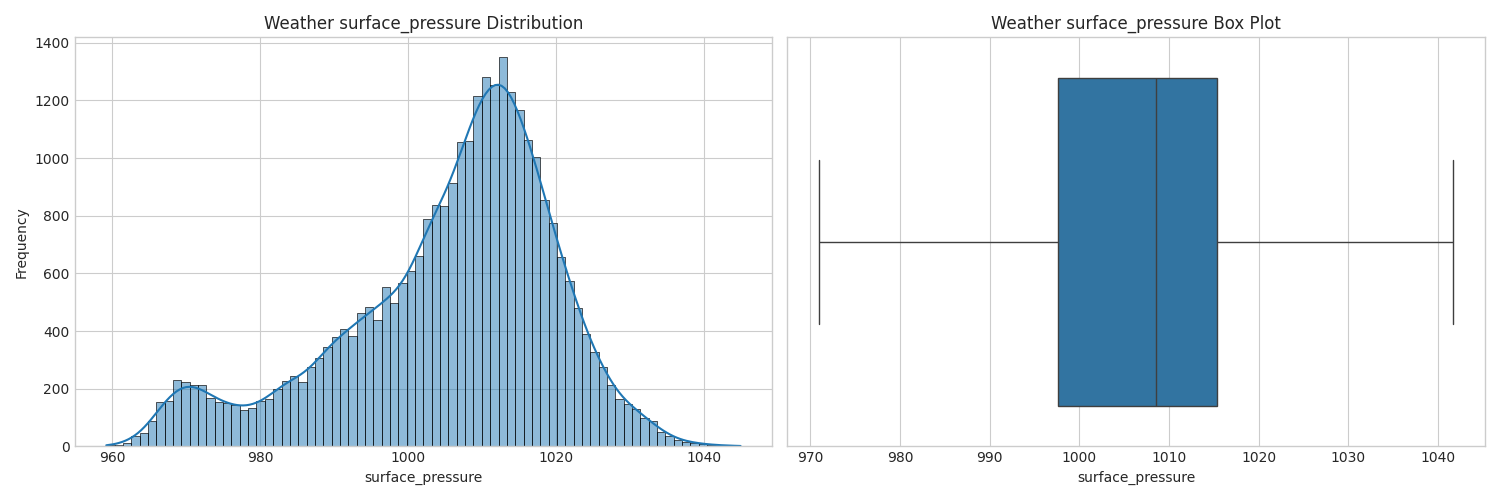
\includegraphics[width=0.8\textwidth]{../plots/weather_distribution_surface_pressure.png}
    \caption{天气分析:地表气压 (surface\_pressure) 分布,形态与海平面气压类似,但数值范围可能因海拔影响而不同。} % Updated caption
    \label{fig:weather_dist_surface_pressure}
\end{figure}

\begin{figure}[H]
    \centering
    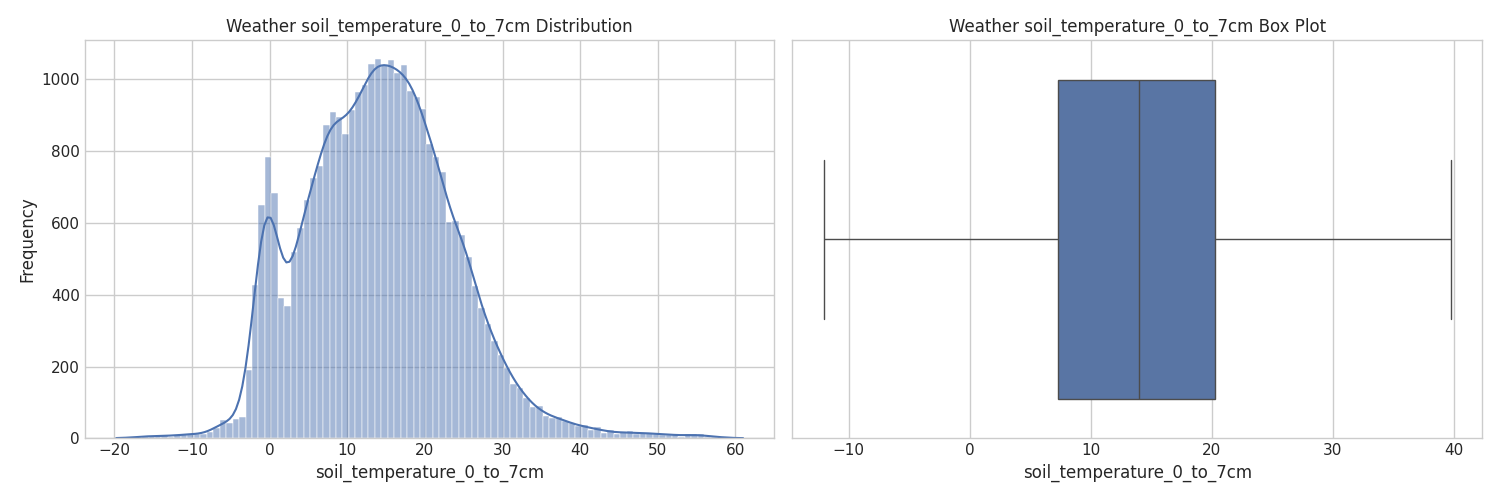
\includegraphics[width=0.8\textwidth]{../plots/weather_distribution_soil_temperature_0_to_7cm.png}
    \caption{天气分析:0-7cm 土壤温度 (soil\_temperature\_0\_to\_7cm) 分布,受气温影响,呈季节性变化。} % Updated caption
    \label{fig:weather_dist_soil_temp}
\end{figure}

\begin{figure}[H]
    \centering
    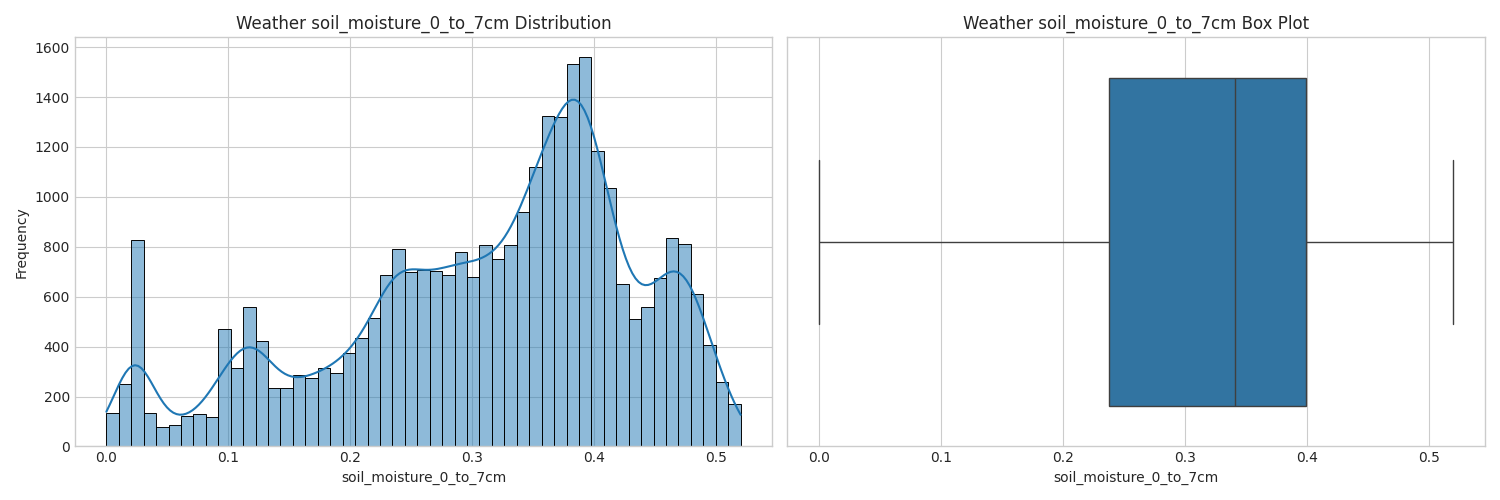
\includegraphics[width=0.8\textwidth]{../plots/weather_distribution_soil_moisture_0_to_7cm.png}
    \caption{天气分析:0-7cm 土壤湿度 (soil\_moisture\_0\_to\_7cm) 分布,反映表层土壤含水量。} % Updated caption
    \label{fig:weather_dist_soil_moisture}
\end{figure}

\begin{figure}[H]
    \centering
    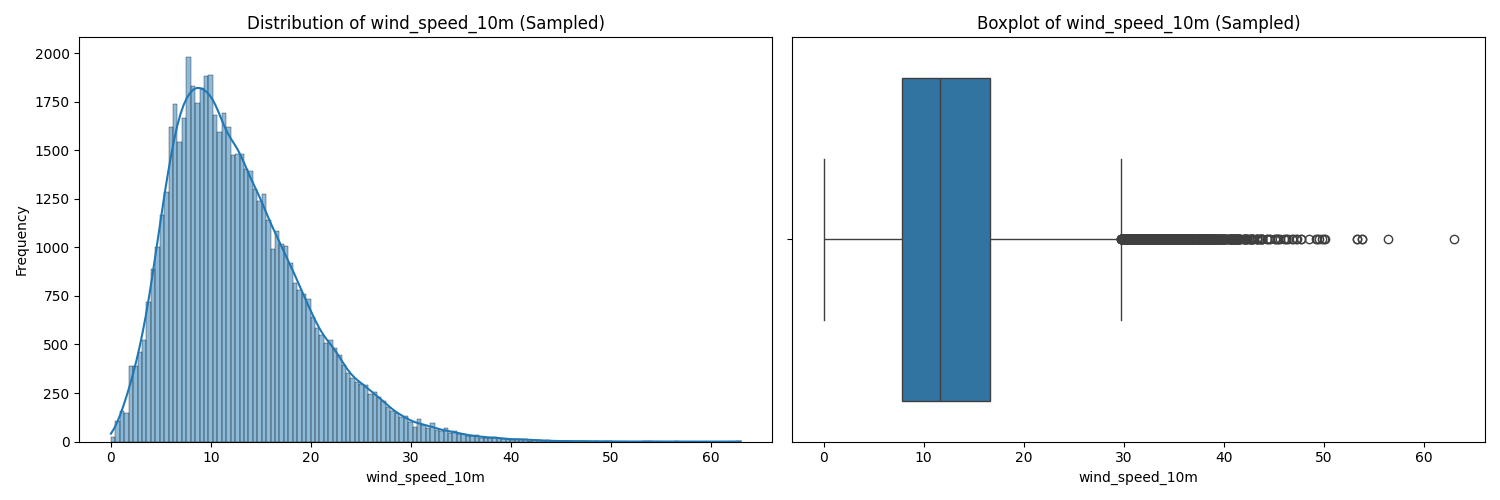
\includegraphics[width=0.8\textwidth]{../plots/weather_distribution_wind_speed_10m.png}
    \caption{天气分析:10 米风速 (wind\_speed\_10m) 分布,右偏分布,多数时间风速较低。} % Updated caption
    \label{fig:weather_dist_wind}
\end{figure}

\begin{figure}[H]
    \centering
    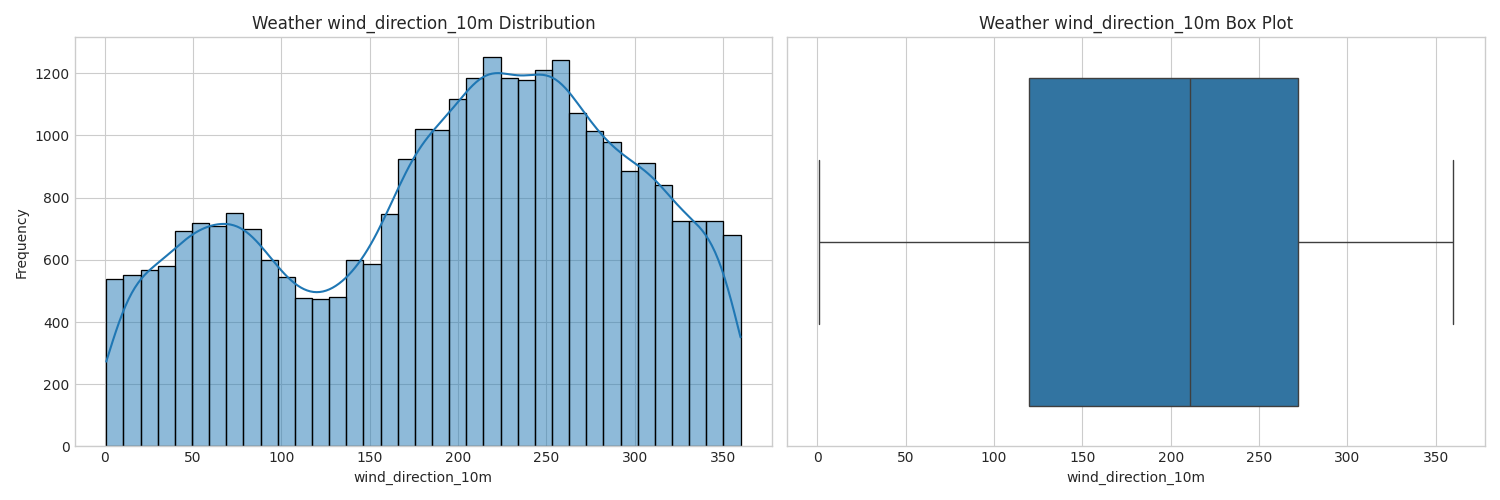
\includegraphics[width=0.8\textwidth]{../plots/weather_distribution_wind_direction_10m.png}
    \caption{天气分析:10 米风向 (wind\_direction\_10m) 分布,可能显示主导风向。} % Updated caption
    \label{fig:weather_dist_wind_dir}
\end{figure}

\begin{figure}[H]
    \centering
    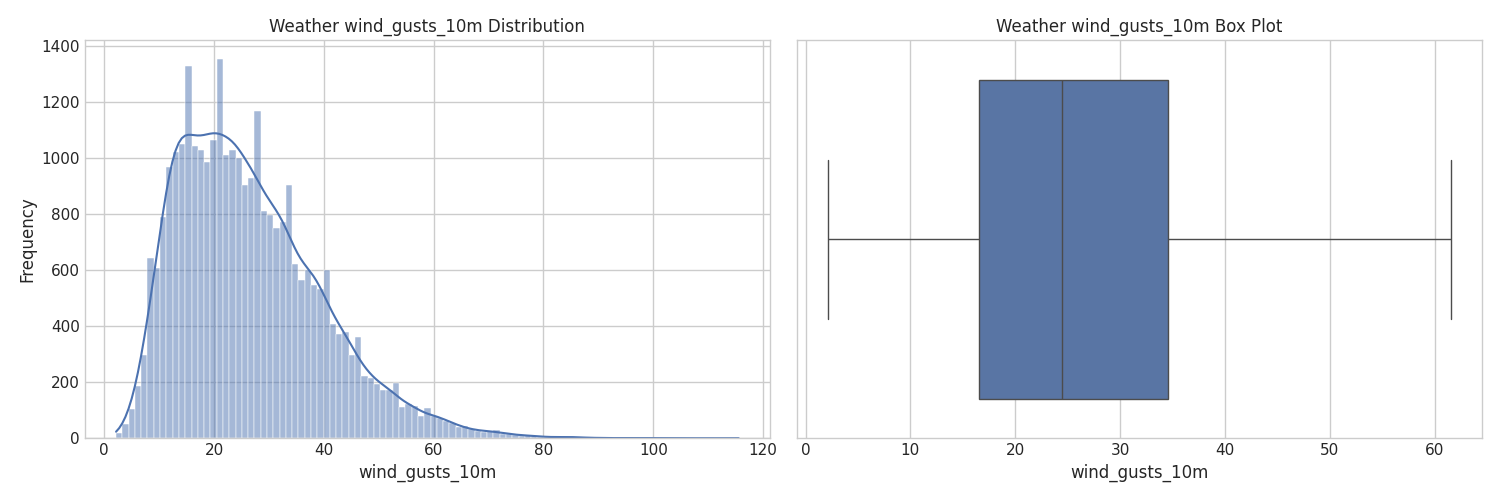
\includegraphics[width=0.8\textwidth]{../plots/weather_distribution_wind_gusts_10m.png}
    \caption{天气分析:10 米阵风速度 (wind\_gusts\_10m) 分布,右偏,反映最大瞬时风速。} % Updated caption
    \label{fig:weather_dist_wind_gusts}
\end{figure}

\begin{figure}[H]
    \centering
    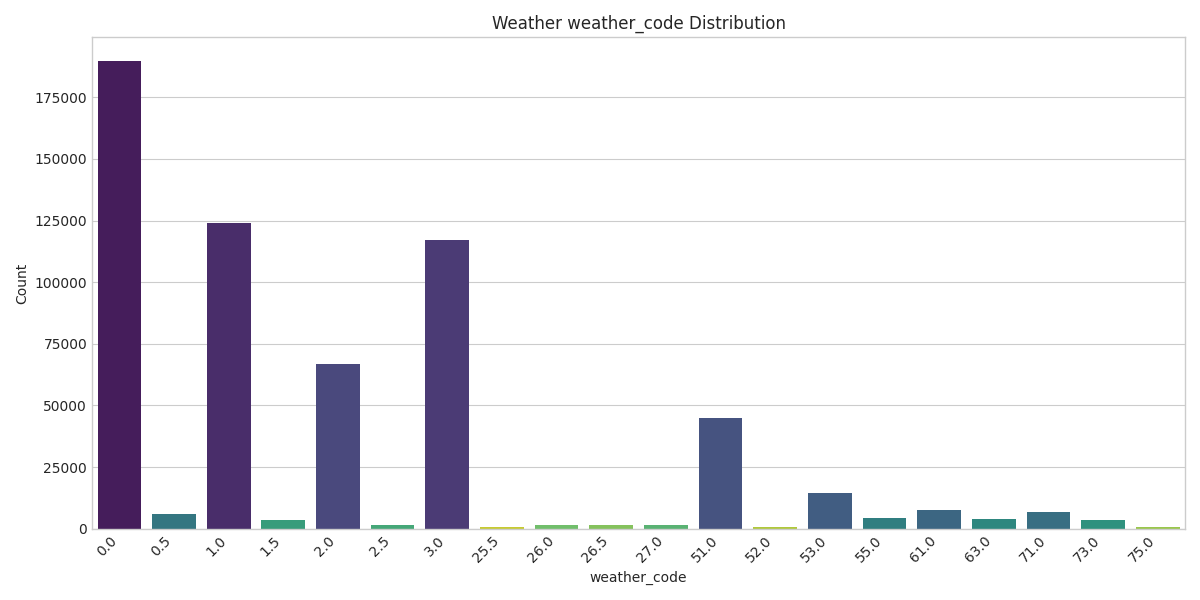
\includegraphics[width=0.8\textwidth]{../plots/weather_distribution_weather_code.png}
    \caption{天气分析:天气代码 (weather\_code) 频率分布(Top 20 及其他),显示最常见的天气类型。} % Updated caption
    \label{fig:weather_dist_code}
\end{figure}

\begin{figure}[H]
    \centering
    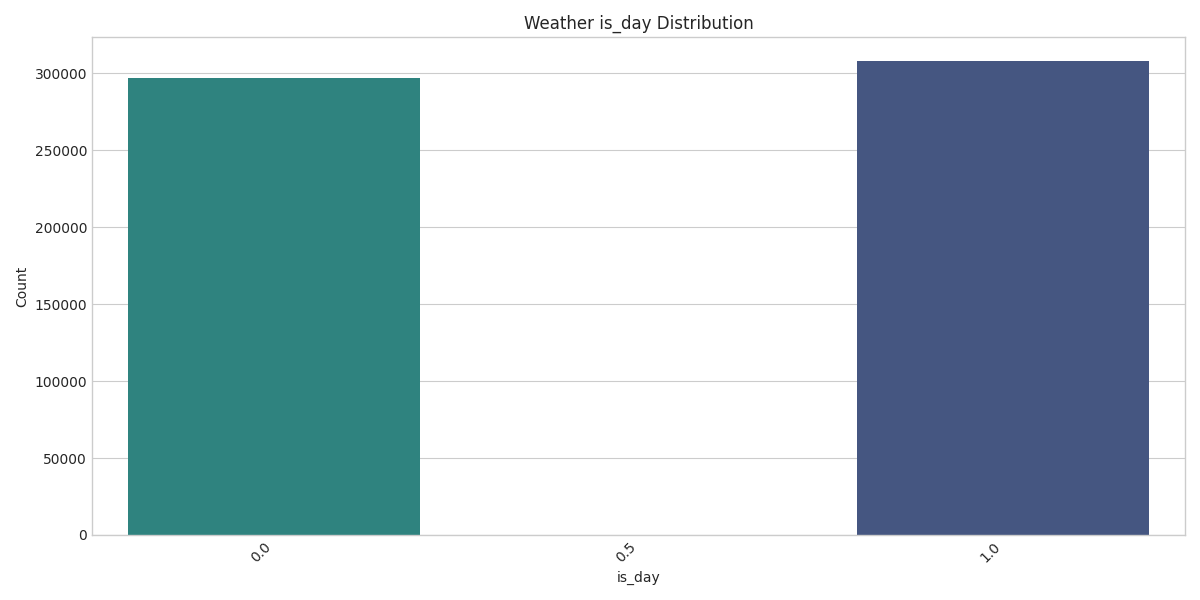
\includegraphics[width=0.6\textwidth]{../plots/weather_distribution_is_day.png}
    \caption{天气分析:"是否白天" (is\_day) 标签分布,白天 (1) 和夜晚 (0) 记录数大致平衡。} % Updated caption
    \label{fig:weather_dist_is_day}
\end{figure}

\begin{figure}[H]
    \centering
    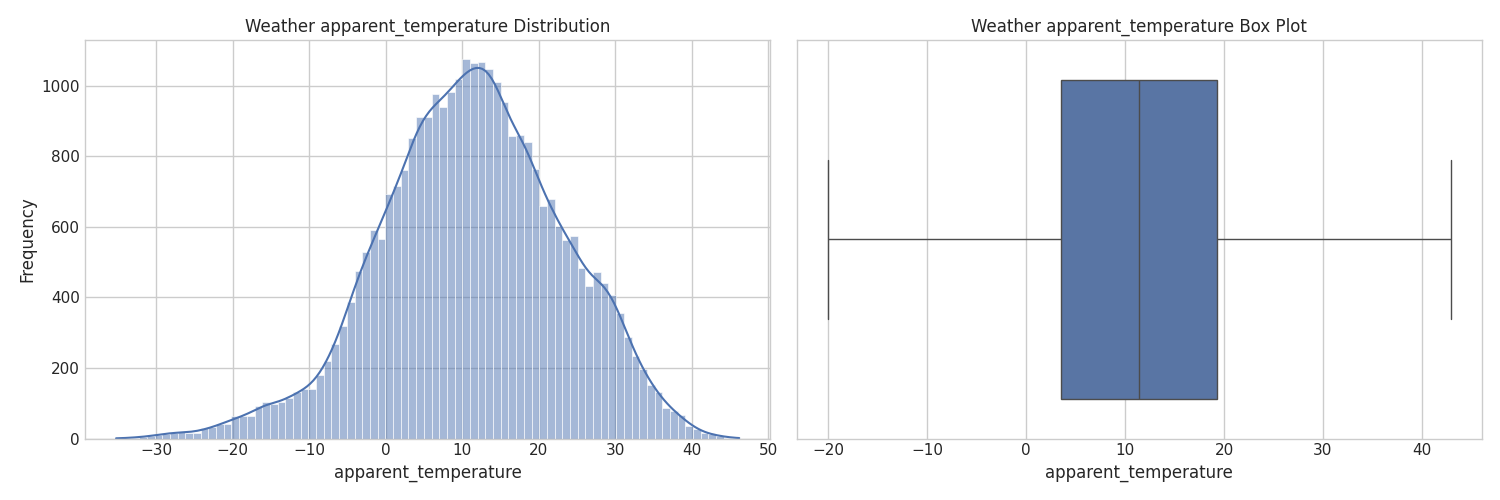
\includegraphics[width=0.8\textwidth]{../plots/weather_distribution_apparent_temperature.png}
    \caption{天气分析:体感温度 (apparent\_temperature) 分布,综合考虑温度、湿度、风速等因素。} % Updated caption
    \label{fig:weather_dist_apparent_temp}
\end{figure}

\section{关系分析}
\label{sec:relationship_analysis}

本节旨在探索电力需求与元数据、天气特征之间的潜在关系。

\subsection{需求与元数据的关系}
\label{subsec:demand_metadata}

为了研究不同元数据属性(如建筑类型、数据集来源、地理位置)对电力需求的影响,将抽样得到的需求数据子集与元数据表进行合并,并按元数据类别进行分组比较。使用箱线图(如图 \ref{fig:demand_vs_building_class_orig}, \ref{fig:demand_vs_dataset_orig}, \ref{fig:demand_vs_location_orig} 等)在原始尺度和对数变换尺度下展示了不同类别下电力需求分布的差异。分析结果清晰地显示,例如,商业建筑的电力需求显著高于住宅建筑;不同来源的数据集或不同地理位置对应的需求分布也存在明显差异。

\begin{figure}[H]
    \centering
    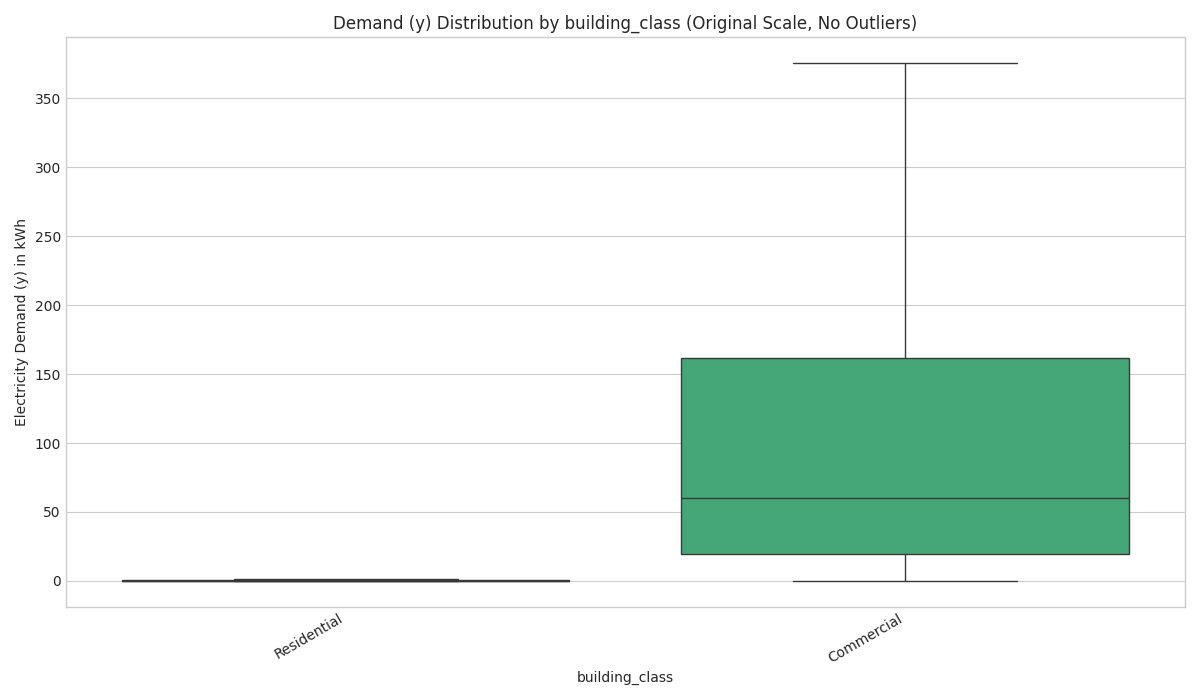
\includegraphics[width=0.8\textwidth]{../plots/demand_vs_building_class_boxplot_orig.png}
    \caption{电力需求 (y) 与建筑类型 (building\_class) 的关系(原始尺度,移除部分离群点):箱线图清晰展示商业建筑的需求显著高于住宅建筑。} % Updated caption
    \label{fig:demand_vs_building_class_orig}
\end{figure}

\begin{figure}[H]
    \centering
    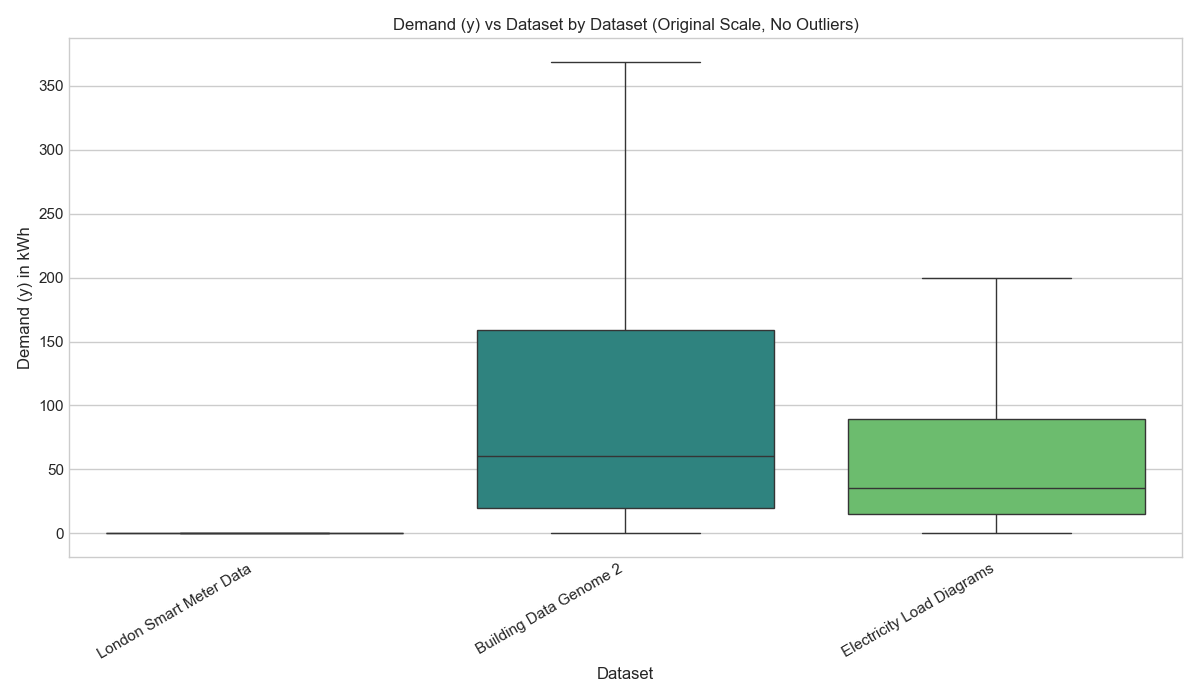
\includegraphics[width=0.8\textwidth]{../plots/demand_vs_dataset_boxplot_orig.png}
    \caption{电力需求 (y) 与数据集来源 (dataset) 的关系(原始尺度):箱线图显示不同来源数据集的需求分布存在差异。} % Updated caption
    \label{fig:demand_vs_dataset_orig}
\end{figure}

\begin{figure}[H]
    \centering
    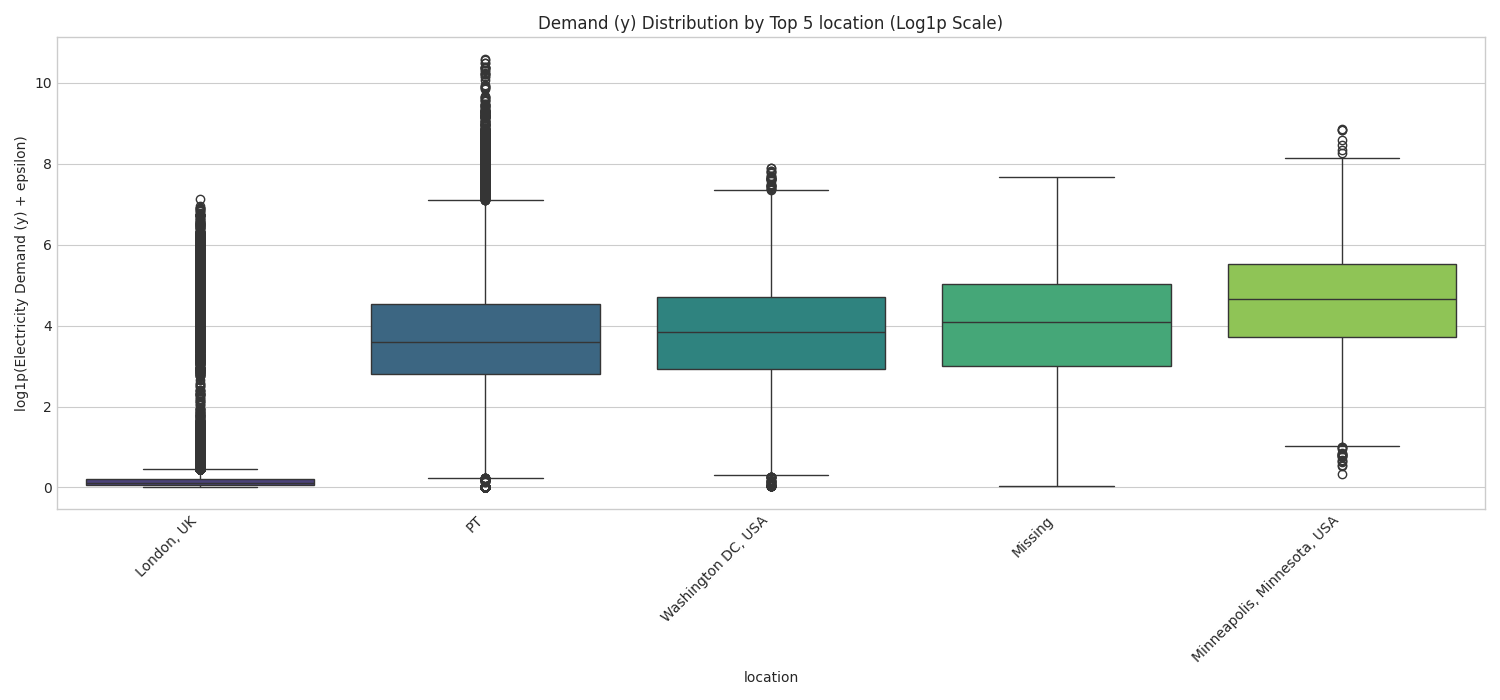
\includegraphics[width=0.8\textwidth]{../plots/demand_vs_top5_location_boxplot_log1p.png}
    \caption{电力需求 (y) 与主要地理位置 (location) 的关系(log1p 变换尺度):比较 Top 5 地点在对数尺度下的需求分布。} % Updated caption
    \label{fig:demand_vs_location_log}
\end{figure}

\begin{figure}[H]
    \centering
    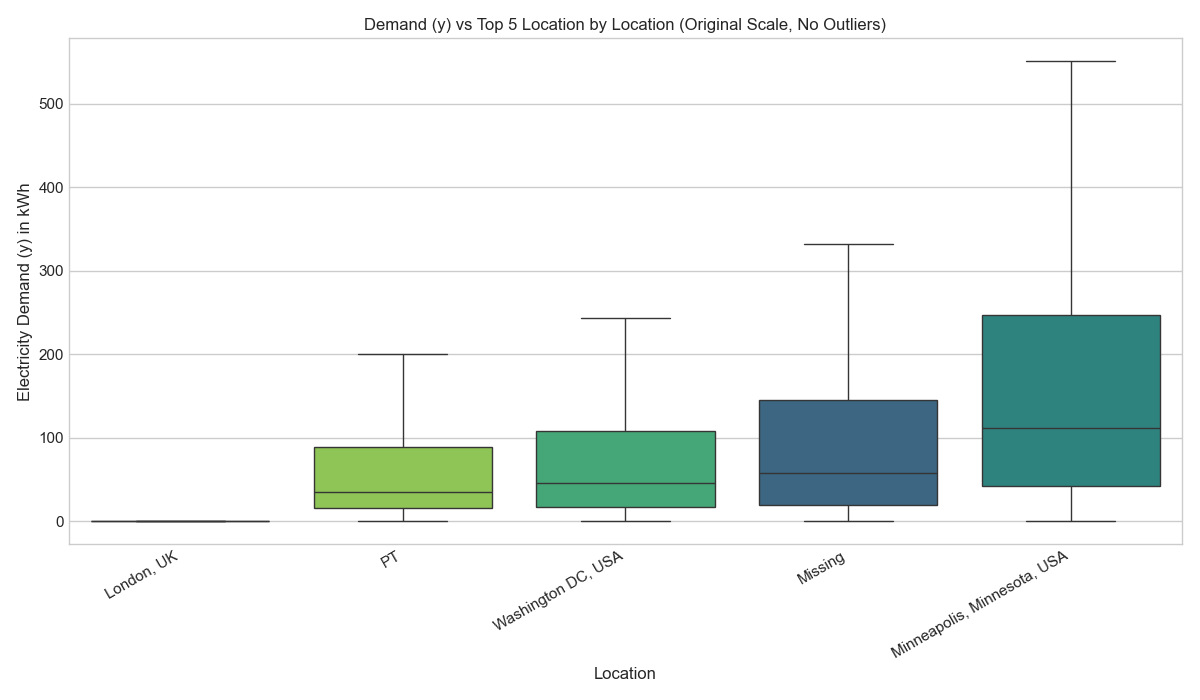
\includegraphics[width=0.8\textwidth]{../plots/demand_vs_top5_location_boxplot_orig.png}
    \caption{电力需求 (y) 与主要地理位置 (location) 的关系(原始尺度):比较 Top 5 地点在原始尺度下的需求水平和变异性。} % Updated caption
    \label{fig:demand_vs_location_orig}
\end{figure}

\subsection{需求与天气的关系及数据合并}
\label{subsec:demand_weather}

为量化天气因素对电力需求的影响,并为后续建模准备统一的数据集,执行了数据合并流程。该过程主要步骤如下:
\begin{enumerate}
    \item \textbf{加载数据}: 加载经过处理(如重采样至小时频率)的需求数据、元数据和天气数据。
    \item \textbf{初步合并}: 将需求数据与元数据通过监测点唯一标识符进行连接,保留所有需求记录,并选取必要的元数据字段(如地理位置标识符、建筑类型)。
    \item \textbf{时间戳对齐与天气数据准备}: 将合并后数据的时间戳统一处理到小时级别,作为与天气数据连接的时间键。同时,对天气数据按地理位置标识符和时间戳进行去重处理,移除了少量重复记录。
    \item \textbf{最终合并与诊断}: 将处理后的需求 - 元数据表与去重后的天气数据表,使用地理位置标识符和小时级时间戳作为键进行左连接,将天气信息附加到对应的需求记录上。
    \item \textbf{诊断分析发现}: 合并过程中发现,由于元数据中存在一个无法在天气数据中匹配到的地理位置标识符,以及一个 NULL 的地理位置标识符,导致最终合并的数据集中约有 1.73\% 的记录未能成功关联到天气信息,其天气相关字段为空值。对于具有有效且可匹配地理位置标识符的记录,天气数据连接成功率非常高。
\end{enumerate}
该合并流程生成了一个包含对齐的需求、元数据和天气信息的宽表数据集,为后续的特征工程和模型训练奠定了基础。

初步的相关性分析(基于抽样数据)表明,电力需求与某些天气变量(特别是温度、湿度、体感温度、云量)存在较明显的相关性。此外,为了解天气变量内部的相互关系,计算并可视化了数值型天气特征之间的相关性矩阵(见图 \ref{fig:weather_correlation}),发现许多天气变量之间本身存在强相关性(例如,温度与体感温度、露点温度高度相关),这提示在建模时可能需要关注多重共线性问题。

\begin{figure}[H]
    \centering
    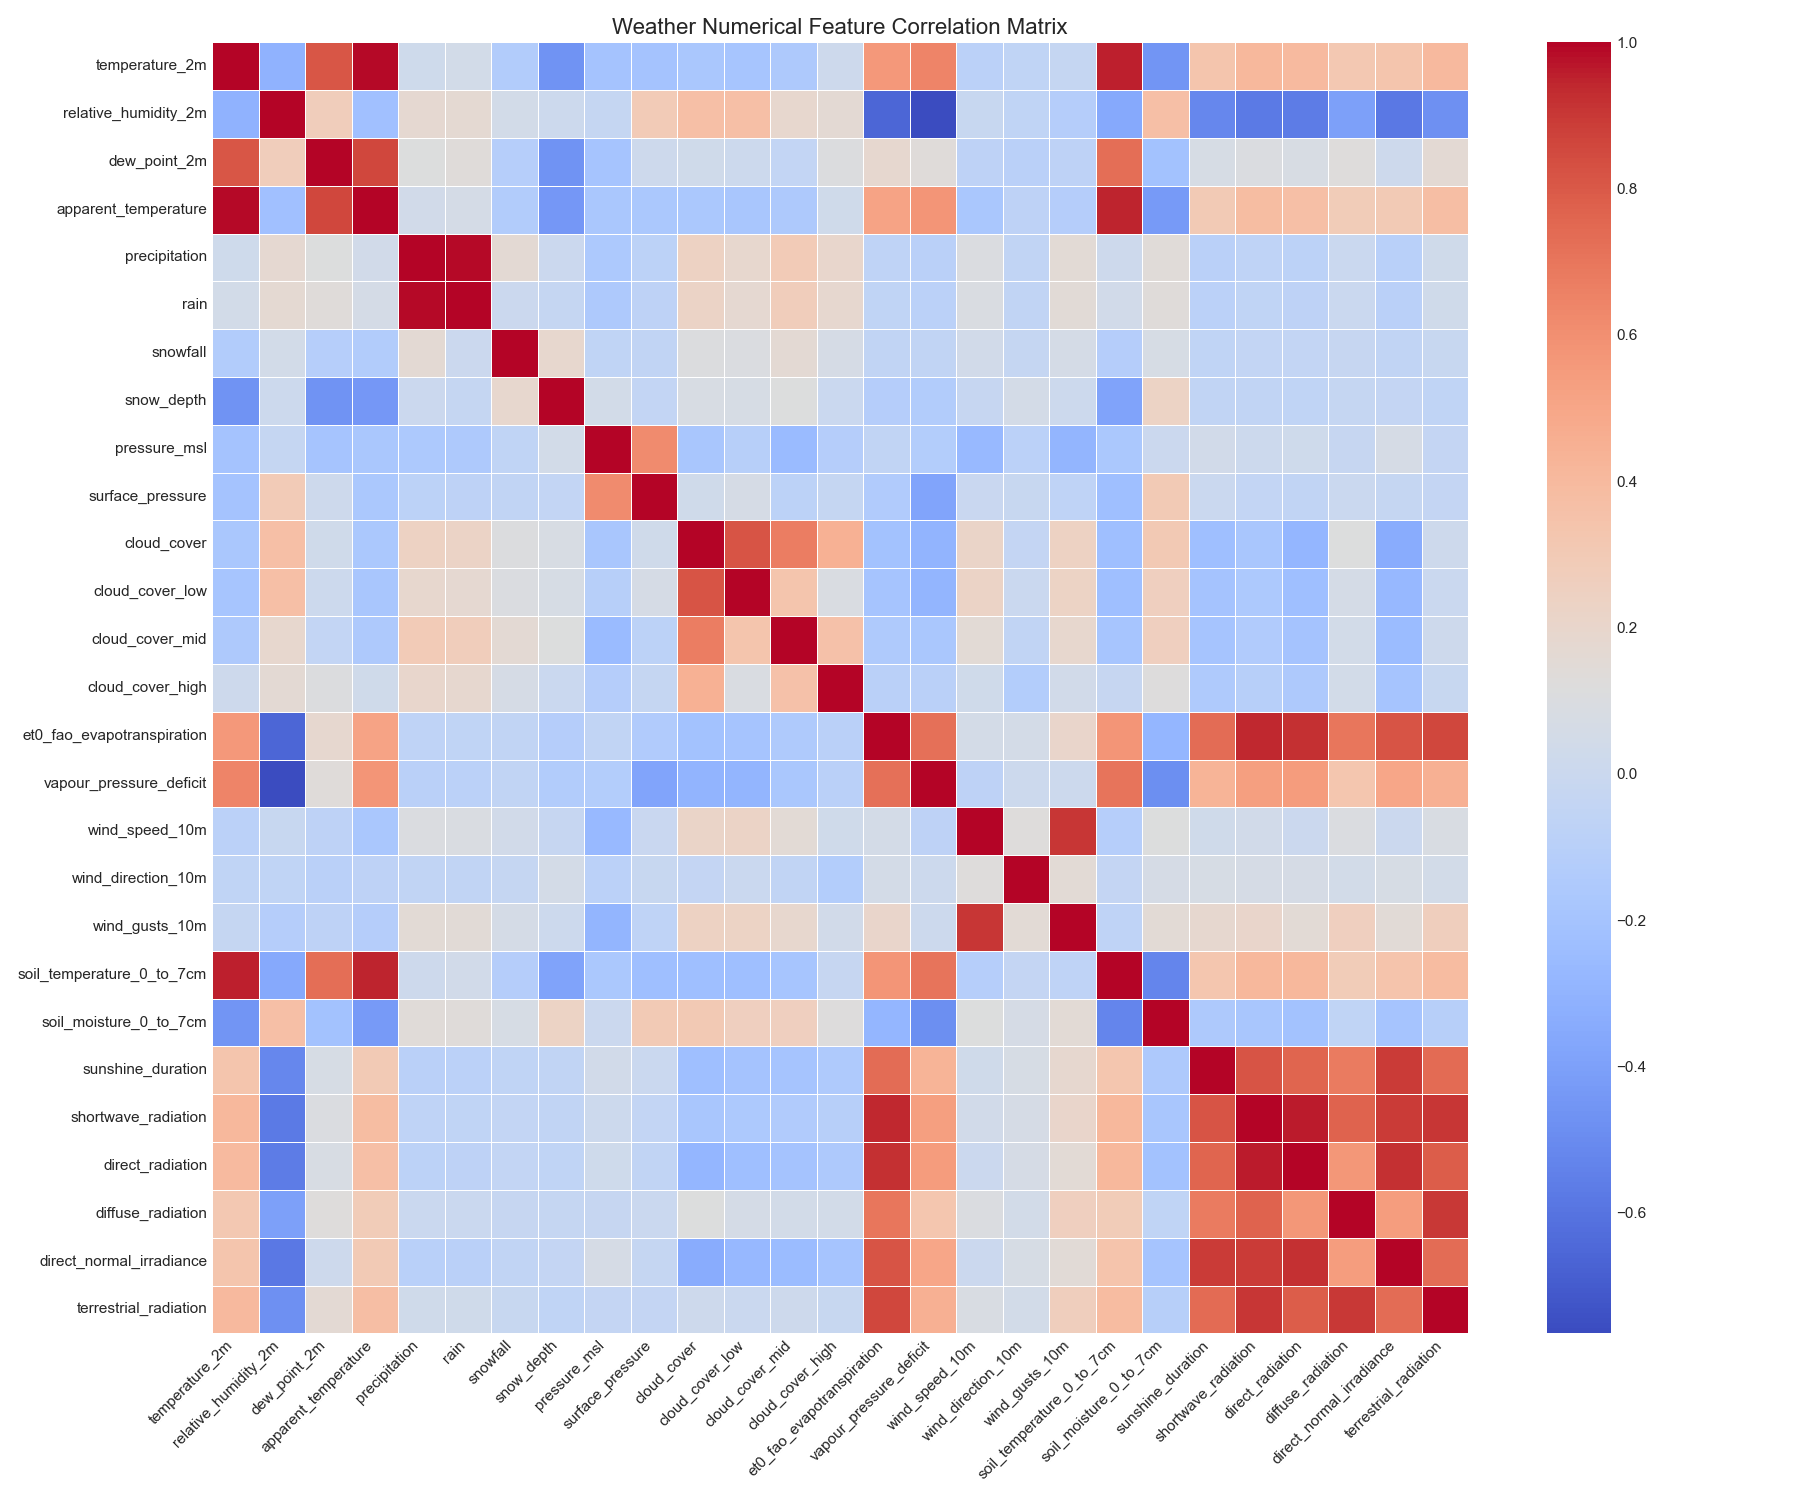
\includegraphics[width=0.9\textwidth]{../plots/weather_correlation_matrix.png}
    \caption{数值型天气特征相关性矩阵热力图:揭示了天气变量之间的线性关联强度和方向,提示了潜在的多重共线性问题(如温度相关变量之间的高度相关性)。} % Updated caption
    \label{fig:weather_correlation}
\end{figure}

\section{时间特征分析}
\label{sec:time_analysis}

本节深入分析数据的时间维度特性。

\subsection{时间戳频率分析与匹配实现}
\label{sec:frequency_matching}

通过计算相邻记录间的时间差,分析了需求数据和天气数据各自的时间戳采样频率。需求数据存在多种主要的采样间隔(如 15 分钟、30 分钟、1 小时),而天气数据主要为 1 小时间隔。这种时间粒度上的不一致性在数据准备阶段通过以下策略解决:首先,将原始需求数据统一重采样到小时频率,聚合得到每小时的总需求量;其次,在合并需求数据和天气数据时,将需求数据的时间戳调整至小时级别,然后与天气数据的小时级时间戳进行匹配。通过这种方式,成功地将不同频率的数据源在统一的时间基准上进行了融合。

\subsection{周期性分析}
\label{sec:periodicity_analysis}

为了量化电力需求的周期性模式,从时间戳中提取了时间特征(如小时、星期几、月份),并按这些特征对整个需求数据集进行分组,计算每个时间组的平均电力需求。将结果绘制成图表(如图 \ref{fig:demand_by_hour}, \ref{fig:demand_by_dayofweek}, \ref{fig:demand_by_month})。分析结果清晰地展示了:
\begin{itemize}
    \item \textbf{小时周期} (图 \ref{fig:demand_by_hour}): 平均需求呈现典型的日内变化模式,具有白天高峰和夜间低谷。
    \item \textbf{星期周期} (图 \ref{fig:demand_by_dayofweek}): 工作日和周末的平均需求存在显著差异。
    \item \textbf{月份周期} (图 \ref{fig:demand_by_month}): 平均需求呈现明显的季节性波动,通常冬季和夏季较高。
\end{itemize}
这些确凿的周期性是构建时间序列预测模型时必须考虑和利用的关键信息。

\begin{figure}[H]
    \centering
    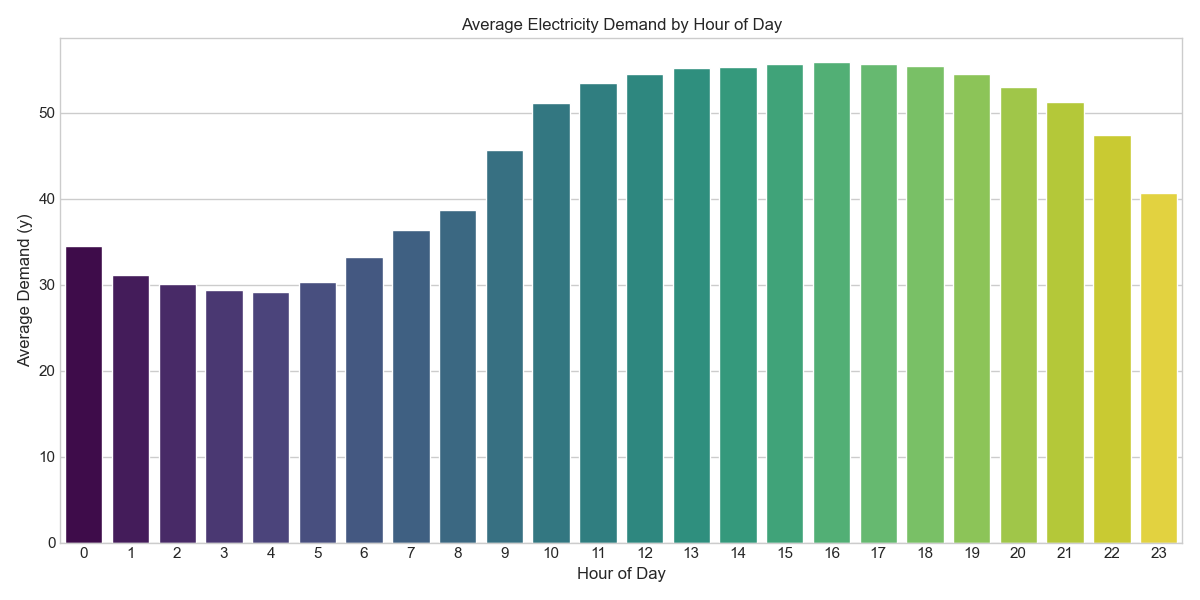
\includegraphics[width=0.8\textwidth]{../plots/avg_demand_by_hour_spark.png}
    \caption{按小时聚合的平均电力需求:条形图清晰展示了日内周期性模式,白天需求高,夜间需求低。} % Updated caption
    \label{fig:demand_by_hour}
\end{figure}

\begin{figure}[H]
    \centering
    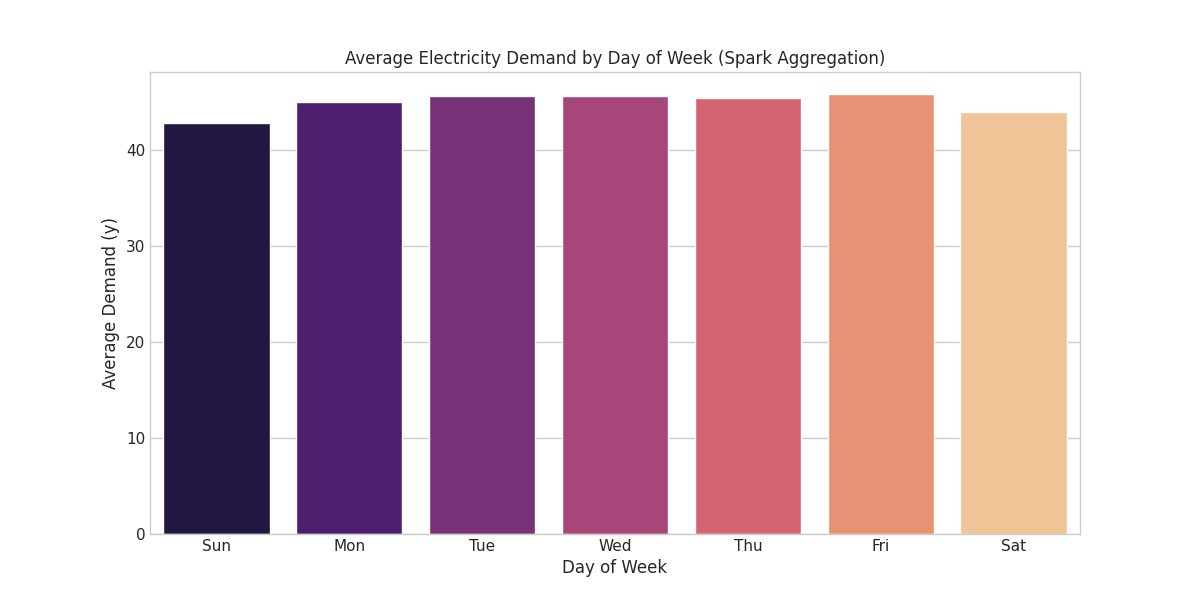
\includegraphics[width=0.8\textwidth]{../plots/avg_demand_by_dayofweek_spark.png}
    \caption{按星期几聚合的平均电力需求:条形图展示了周内周期性模式,工作日与周末的需求模式存在差异。} % Updated caption
    \label{fig:demand_by_dayofweek}
\end{figure}

\begin{figure}[H]
    \centering
    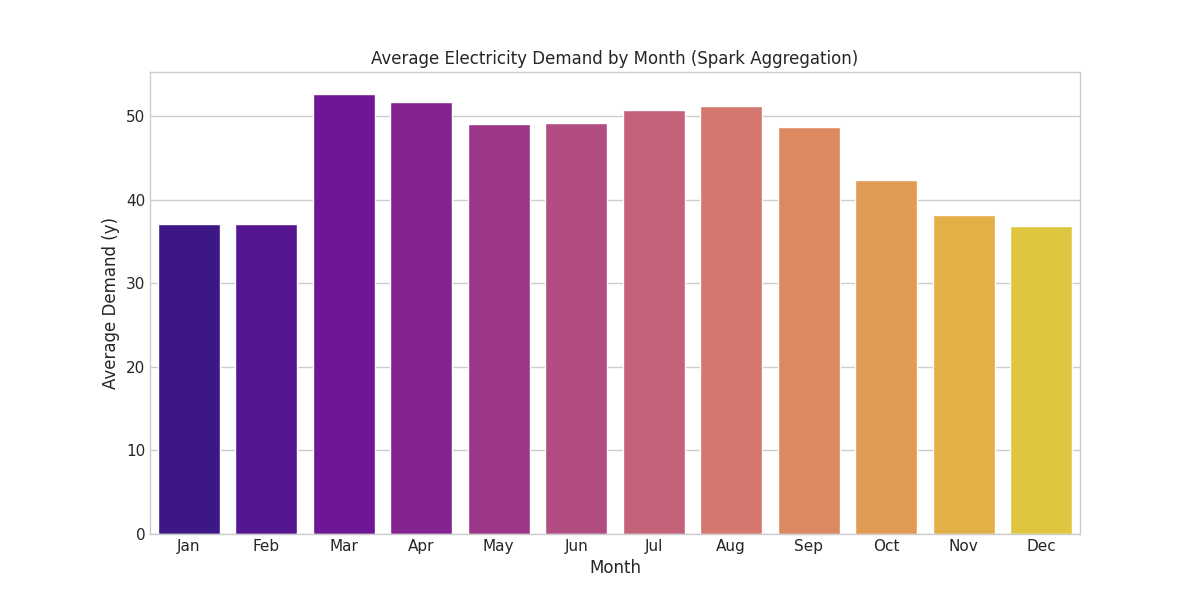
\includegraphics[width=0.8\textwidth]{../plots/avg_demand_by_month_spark.png}
    \caption{按月份聚合的平均电力需求:条形图展示了季节性周期性模式,反映了年度的需求波动规律。} % Updated caption
    \label{fig:demand_by_month}
\end{figure}

\section{特征工程}
\label{sec:feature_engineering}

在完成初步的数据探索和合并之后,进行了特征工程,旨在从现有数据中提取和构建更有预测能力的特征,为后续的机器学习模型训练做准备。主要步骤如下:

\subsection{时间特征提取}
\label{subsec:time_features}
为使模型能够捕捉数据中固有的周期性模式,从合并后数据的时间戳列中提取了多个时间维度特征,包括:年份、月份、日期、星期几、年内第几天以及小时。这些特征直接反映了需求发生的时间上下文。

\subsection{滚动窗口统计特征}
\label{subsec:rolling_features}
为捕捉电力需求 (y) 的近期动态变化和局部趋势,计算了一系列基于滑动时间窗口的历史统计特征。这些特征基于每个监测点自身过去一段时间的需求表现。定义了多个回顾性时间窗口(例如,3 小时、6 小时、12 小时、24 小时、48 小时、168 小时),并在每个窗口内计算了需求值的均值、标准差、最小值和最大值。这些特征有助于模型理解需求的短期波动和趋势。

\subsection{缺失值处理}
\label{subsec:fe_missing_values}
特征工程过程中处理了潜在的缺失值:
\begin{enumerate}
    \item \textbf{移除目标缺失行}: 直接删除了目标变量 y 本身就缺失的记录。
    \item \textbf{移除初始窗口期数据}: 由于滚动窗口特征需要依赖历史数据,每个时间序列最初的若干时间点无法计算出有效的滚动特征值(导致这些特征列在此期间为空)。基于最大回顾窗口期的特征可用性,移除了这些初始时间点的记录,确保用于建模的数据具有完整的历史滚动信息。
\end{enumerate}

\subsection{特征集输出}
\label{subsec:fe_optimization_output}
最终,将包含原始合并信息、新增时间特征和滚动统计特征的数据集进行保存。为了便于后续按时间范围进行高效的数据加载和模型训练/评估,输出数据在物理存储上按照年份和月份进行了分区。生成的特征集包含了丰富的时间上下文信息和需求动态信息,为后续的模型训练和预测任务奠定了数据基础。

\section{总结与后续步骤}
\label{sec:conclusion}

本次探索性数据分析与特征工程揭示了该电力需求数据集的关键特征、数据质量问题、重要模式和关系,并为建模准备了特征集:
\begin{itemize}
    \item 数据集包含大规模、多来源的异构数据,已通过适当的数据处理技术完成合并与特征提取。
    \item 数据质量方面,需关注电力需求目标值的少量缺失(已处理)、部分元数据(特别是地理位置标识符)的缺失或不匹配问题(导致合并后约 1.73\% 的记录天气信息缺失)、以及天气数据中的少量重复记录(已处理)。
    \item 电力需求值呈现高度右偏分布,包含极端值。
    \item 元数据中的分类信息(如建筑类型、地理位置)与电力需求水平显著相关。
    \item 天气因素(尤其是温度、湿度等)与电力需求存在明确的相关性。
    \item 电力需求表现出清晰的多重时间周期性(日、周、年),已通过提取时间特征和滚动特征加以捕捉。
    \item 不同数据源间的时间采样频率不匹配问题已通过重采样和时间戳对齐策略解决。
    \item 特征工程阶段生成了时间特征和多窗口滚动统计特征,并处理了目标变量缺失和滚动窗口初始期缺失的问题。最终特征集已按时间分区存储。
\end{itemize}

基于以上分析和处理,后续的数据处理和建模工作的建议方向包括:
\begin{enumerate}
    \item \textbf{数据清洗与预处理 (针对特征数据)}:
        \begin{itemize}
            \item 处理合并后数据中因地理位置标识符问题导致的天气数据缺失(约 1.73\% 的行),可考虑插补或移除这些行。
        \end{itemize}
    \item \textbf{进一步特征工程 (可选)}:
        \begin{itemize}
            \item 创建滞后特征(Lag Features):将目标变量 y 或重要特征(如温度)在过去特定时间点的值作为当前时间点的特征。
            \item 创建交互特征(Interaction Features):例如,温度与小时的交互,可能有助于捕捉不同时间段温度对需求影响的差异。
            \item 对分类特征(如建筑类型、星期几、小时等)进行适合模型的编码(如独热编码、目标编码)。
            \item 根据所选模型的需求,对数值特征进行必要的变换(如对数变换以缓解偏度)或标准化/归一化。
        \end{itemize}
    \item \textbf{模型构建准备}:
        \begin{itemize}
            \item 根据时间和监测点 ID 合理划分训练集、验证集和测试集,采用时序交叉验证等方法以避免数据泄露。
        \end{itemize}
    \item \textbf{模型选择与评估}:
        \begin{itemize}
            \item 根据预测目标和数据特性选择合适的时间序列预测模型(如统计模型 ARIMA、指数平滑,机器学习模型 LightGBM、XGBoost,或深度学习模型 RNN、Transformer 等)。
            \item 建立包含特征处理、模型训练和评估的完整流程(pipeline)。
            \item 选择合适的评估指标(如 RMSE, MAE, MAPE)并在验证集上进行模型选择和超参数调优。
        \end{itemize}
\end{enumerate}

本报告的探索性分析和特征工程为理解数据特性和指导后续建模流程奠定了基础。

\end{document}
